% Provenance (never printed): see sources/outline_sources.md (Year 3: primordial
% nucleosynthesis and stellar burning recalled from the physics books; the s and r
% processes; supernovae and neutron-star mergers; galactic chemical evolution; from the
% solar abundances to the composition of the Earth).
% Brief: sources/book5/BRIEFS.md, ch. 30. Curves from figdata/bachelor-3/
% solar_abundances.py (Asplund, Amarsi और Grevesse 2021, Table 2), neutron_capture.py
% (their Table B.1 isotopes, KADoNiS v0.3 cross sections, IAEA Live Chart half-lives) and
% chemical_evolution.py (closed box against the Geneva-Copenhagen survey of Casagrande et
% al. 2011, and a two-phase [alpha/Fe] model). Exercise and problem values in the Book 5
% scratch calculator calc/ch30.py.
\chapter{तत्त्व कहाँ से आते हैं}\label{ch:b3:origin-of-elements}

चूना-पत्थर की एक कगार का कैल्शियम अधिकतर उन विशाल तारों के भीतर बना था,
जो सूर्य के जन्म से पहले विस्फोटित हो चुके थे। पृथ्वी के क्रोड का लोहा
मुख्य रूप से एक भिन्न प्रकार के विस्फोट से आता है, अर्थात
श्वेत वामन के विस्फोट से। एक अंगूठी का प्लैटिनम प्रचुरता के उस शिखर का है
जो सेकंडों तक चलने वाली \omterm{def:b3:origin-of-elements:s-process}{न्यूट्रॉन प्रग्रहण} की बौछारों से बना है, दो न्यूट्रॉन तारों के
विलय में, या किसी दुर्लभ प्रकार के अधिनवतारा में; इन दोनों में से किसने उसका अधिकांश
बनाया, यह अब भी विवादित है।
इनमें से हर घटना ने सूर्य के संघटन पर अपनी छाप छोड़ी है,
जो, उन थोड़े-से तत्त्वों को छोड़कर जिन्हें ग्रह अपने पास रख नहीं पाए, वही
सौरमंडल का भी संघटन है। यह अध्याय उस अभिलेख को पढ़ता है:
सौर प्रचुरताएँ प्रस्तुत करता है, याद दिलाता है कि हल्के तत्त्व कैसे बने,
भारी तत्त्वों को गढ़ने वाले न्यूट्रॉन प्रग्रहणों का अनुसरण करता है, और
हर प्रक्रम कहाँ चलता है, वे स्थल खोजता है, और मॉडल बनाता है कि किसी
मंदाकिनी का संघटन उसके तारों के जन्म और मृत्यु के साथ कैसे बदलता है। यह वहाँ समाप्त होता है जहाँ
पिछली पुस्तकों का भूविज्ञान आरंभ होता है: पृथ्वी, जो सूर्य के ही पदार्थ से बनी है,
लोहे से इतनी समृद्ध और वाष्पशीलों में इतनी निर्धन क्यों है।
% ledger: matteucci21:production, cowan21:rprocess, kobayashi20:origins, asplund21:fig1

\begin{recall}
बिग बैंग न्यूक्लियोसंश्लेषण, तारों में हाइड्रोजन और हीलियम का संलयन,
प्रति न्यूक्लियॉन बंधन-ऊर्जा और लोहे के निकट उसका उच्चिष्ठ, स्थिरता की
घाटी, बीटा क्षय और अर्ध-आयु, किसी अभिक्रिया का अनुप्रस्थ-काट,
मुख्य अनुक्रम के तारे, लाल दानव, श्वेत वामन, न्यूट्रॉन तारे और
अधिनवतारे भौतिकी की पुस्तकों में हैं। उल्कापिंडों के वर्ग, CI
कॉन्ड्राइट, संघनन तापमान, दुर्गलनीय और वाष्पशील
तत्त्व, गोल्डश्मिट वर्ग और समग्र सिलिकेट पृथ्वी, ये सब
पुस्तक 4 (स्नातक वर्ष 2) में, उसके ग्रहों की संरचना और
पृथ्वी के तत्त्वों पर अध्यायों में ये हैं। आकाशगंगा की संरचना, उसकी पतली और
मोटी चक्रिकाएँ, उसका प्रभामंडल और उसकी तारकीय समष्टियाँ पिछले
अध्याय में हैं।
\end{recall}

\section{सौर प्रचुरताएँ}\label{sec:b3:origin-of-elements:solar}

सूर्य, सौरमंडल के द्रव्यमान का \qty{99.85}{\percent} से अधिक धारण करता है,
और उसकी बाहरी परतों ने कुछ हल्के तत्त्वों और भारी तत्त्वों के धीमे अवसादन को छोड़कर,
उस गैस का संघटन बनाए रखा है जिससे
सूर्य और ग्रह बने थे। इसका संघटन दो प्रकार से पढ़ा जाता है:
उसके प्रकाशमंडल की अवशोषण रेखाओं से, और CI कॉन्ड्राइट से, यानी
उन उल्कापिंडों से जिनका संघटन, सबसे वाष्पशील
तत्त्वों को छोड़कर, ज्ञात सभी पदार्थों में सूर्य के सबसे निकट है।
% ledger: asplund21:fig1, asplund21:ci

\begin{definition}[सौर प्रचुरता; डेक्स]\label{def:b3:origin-of-elements:abundance}
किसी तत्त्व $X$ की \emph{सौर प्रचुरता}\index{सौर प्रचुरता} सूर्य में
हाइड्रोजन के परमाणुओं के सापेक्ष उसके परमाणुओं की संख्या है, जो
एक लघुगणकीय पैमाने पर लिखी जाती है, जिस पर हाइड्रोजन को $12$ पर रखा जाता है:
\[
\log\varepsilon(X) = 12 + \log_{10}\frac{N_X}{N_\mathrm{H}} .
\]
ऐसे लघुगणक में एक इकाई के अंतर को
\emph{डेक्स}\index{डेक्स} कहते हैं: जो दो प्रचुरताएँ $0.3$~डेक्स से भिन्न हैं, वे
एक गुणक से भिन्न होती हैं, जो $10^{0.3} \approx 2$ है। किसी तारे के लिए सूर्य के सापेक्ष
प्रचुरता कोष्ठकों के साथ लिखी जाती है:
$[X/\mathrm{H}] = \log_{10}(N_X/N_\mathrm{H})_\star -
\log_{10}(N_X/N_\mathrm{H})_\odot$, और इसी प्रकार $[X/Y]$ किन्हीं भी दो
तत्त्वों के लिए।
\end{definition}

नीचे दिया चित्र उस नवीन संकलन की सौर प्रचुरताएँ दिखाता है
जिसमें सभी 83 दीर्घजीवी तत्त्वों का पुनर्मूल्यांकन हुआ है। लोहा, जिसका
$\log\varepsilon = 7.46$ है, वह हर \num{34700} हाइड्रोजन परमाणुओं के लिए एक परमाणु रखता है;
हीलियम में प्रति हाइड्रोजन परमाणु \num{0.0820} परमाणु हैं। कई
विशेषताएँ उभरकर सामने आती हैं, और अध्याय का शेष भाग उन्हें समझाता है।
% ledger: asplund21:abstract, asplund21:ci, data:b5-asplund21

\begin{omfigure}
\centering
\begin{tikzpicture}
\begin{axis}[width=0.95\linewidth, height=8.4cm, xmin=0, xmax=94,
  ymin=-1.8, ymax=12.8, xlabel={परमाणु क्रमांक $Z$},
  ylabel={$\log\varepsilon(X)$ \;($\log\varepsilon(\mathrm{H}) = 12$)},
  tick label style={font=\scriptsize}, label style={font=\small},
  legend style={font=\scriptsize, at={(0.5,-0.17)}, anchor=north,
    legend columns=2, draw=none, cells={anchor=west},
    /tikz/every even column/.append style={column sep=1em}}]
\addplot[blue!70!black, mark=*, mark size=1.3pt, restrict x to domain=0:84]
  table[x=Z, y=logeps] {figdata/out/bachelor-3-solar_abundances-even.dat};
\addlegendentry{सम $Z$}
\addplot[blue!70!black, mark=*, mark size=1.3pt, restrict x to domain=88:94, forget plot]
  table[x=Z, y=logeps] {figdata/out/bachelor-3-solar_abundances-even.dat};
\addplot[red!70!black, mark=o, mark size=1.4pt]
  table[x=Z, y=logeps] {figdata/out/bachelor-3-solar_abundances-odd.dat};
\addlegendentry{विषम $Z$}
\begin{scope}[font=\scriptsize]
\node[anchor=west] at (axis cs:2.2,12.2) {H};
\node[anchor=west] at (axis cs:3.0,10.9) {He};
\node[anchor=west] at (axis cs:5.6,1.0) {Li, Be, B};
\node[anchor=south] at (axis cs:8,8.95) {O};
\node[anchor=south] at (axis cs:6,8.6) {C};
\node[anchor=south, align=center] at (axis cs:26,7.75) {Fe\\[-1pt]शिखर};
\node[anchor=north] at (axis cs:21,2.95) {Sc};
\node[anchor=south, align=center] at (axis cs:38.5,3.05) {Sr--Zr\\[-1pt]($N = 50$)};
\node[anchor=south] at (axis cs:51.5,2.5) {Te, Xe (r)};
\node[anchor=south, align=center] at (axis cs:58.5,3.7) {Ba\\[-1pt]($N = 82$)};
\node[anchor=south] at (axis cs:76.5,1.95) {Pt (r)};
\node[anchor=south, align=center] at (axis cs:82.5,2.85) {Pb\\[-1pt]($N = 126$)};
\node[anchor=south] at (axis cs:89.6,0.15) {Th};
\node[anchor=north] at (axis cs:92,-0.7) {U};
\end{scope}
\end{axis}
\end{tikzpicture}
\par\smallskip{\small सूर्य में तत्त्वों की प्रचुरताएँ, एक लघुगणकीय पैमाने पर,
जिसमें हाइड्रोजन का मान 12 है: प्रकाशमंडलीय मान, या
उन तत्त्वों के लिए CI कॉन्ड्राइट के मान, जिनकी कोई मापनीय प्रकाशमंडलीय
रेखा नहीं है (Asplund, Amarsi और Grevesse, 2021)। सम और विषम परमाणु क्रमांक
दो रेखाओं के रूप में दिखाए गए हैं। टेक्नीशियम ($Z = 43$) और प्रोमेथियम ($Z = 61$)
का कोई दीर्घजीवी समस्थानिक नहीं है, और बिस्मथ से थोरियम के बीच के
तत्त्वों का भी नहीं है।}\label{fig:b3:origin-of-elements:curve}
\end{omfigure}
% ledger: data:b5-asplund21, asplund21:fig1

\begin{enumerate}
\item हाइड्रोजन और हीलियम लगभग सभी परमाणु बनाते हैं,
  अन्य सभी को मिलाकर उनसे एक हज़ार गुना अधिक हैं; ये दोनों बिग बैंग में बने,
  और हीलियम का कुछ भाग तब से तारों में भी बना है।
\item लिथियम, बेरिलियम और बोरॉन, जो हीलियम के ठीक बाद आते हैं, कार्बन से बहुत नीचे हैं:
  बेरिलियम कार्बन से बारह मिलियन गुना कम प्रचुर है।
\item ऑक्सीजन से भारी तत्त्वों तक प्रचुरताएँ तीव्र गति से घटती हैं, जिनमें
  ऑक्सीजन, लोहे, बेरियम और सीसे के आसपास शिखर हैं,
  और चित्र में अंकित छोटे शिखर भी।
\item सम परमाणु क्रमांक वाले तत्त्व अपने विषम पड़ोसियों से अधिक प्रचुर हैं:
  स्कैंडियम, जो कैल्शियम और टाइटेनियम के बीच है, लगभग \num{1400}
  गुना कैल्शियम से दुर्लभ है और \num{68} गुना टाइटेनियम से। यह
  \emph{सम--विषम प्रभाव} है।
\item लौह शिखर के बाद वक्र समतल हो जाता है: लोहे से सोने तक
  प्रचुरता \num{3.5e6} गुना घटती है, परंतु सोने से सीसे तक वह
  फिर बढ़ती है, ग्यारह गुना।
\end{enumerate}
% ledger: asplund21:fig1, data:b5-asplund21

द्रव्यमान के अनुसार, वर्तमान प्रकाशमंडल में हाइड्रोजन $X = 0.7438$ है,
हीलियम $Y = 0.2423$ है, और बाकी सब $Z = 0.0139$ है। सुधार करने पर
जो भारी तत्त्व सूर्य के बनने के बाद से प्रकाशमंडल के नीचे बैठ गए हैं,
आद्य-सौर मान, यानी उस गैस के, जिससे सूर्य बना,
$X = 0.7121$, $Y = 0.2725$ और $Z = 0.0154$ हैं।
% ledger: asplund21:xyz

\begin{definition}[धात्विकता]\label{def:b3:origin-of-elements:metallicity}
तारे या गैस की \emph{धात्विकता}\index{धात्विकता} उसमें हीलियम से भारी तत्त्वों की
मात्रा है, जिन्हें खगोल विज्ञान में उनकी रसायन चाहे जो हो, धातु कहा जाता है:
द्रव्यमान भिन्न $Z$ के रूप में, या, जैसा कि आम तौर पर मापा जाता है,
सूर्य के सापेक्ष लोहे की प्रचुरता $[\mathrm{Fe/H}]$ के रूप में।
जिस तारे का $[\mathrm{Fe/H}] = -1$ है, उसमें प्रति हाइड्रोजन परमाणु
सूर्य के लोहे का दसवाँ भाग होता है।
\end{definition}

सौर प्रचुरताओं के दो स्रोत उल्लेखनीय रूप से अच्छी तरह मेल खाते हैं। नीचे का चित्र
उन्हें तत्त्व-दर-तत्त्व तुलना करके दिखाता है। 58 तत्त्वों के लिए, जो न
उल्कापिंडों के लिए बहुत वाष्पशील हैं और न सूर्य में नष्ट हुए हैं,
प्रकाशमंडलीय और CI प्रचुरता का भारित माध्य अंतर
है $\num[separate-uncertainty=true]{0.000 \pm 0.007}$~\omterm{def:b3:origin-of-elements:abundance}{डेक्स}। दो समूह
रेखा से हटते हैं। उल्कापिंडों में हाइड्रोजन, हीलियम,
कार्बन, नाइट्रोजन, ऑक्सीजन और उत्कृष्ट गैसें सूर्य की तुलना में कहीं कम हैं:
ये तत्त्व तब गैस में रह गए जब ठोस संघनित हुए। सूर्य में
उल्कापिंडों की तुलना में \num{200} गुना कम लिथियम है: उसने
अपने नाभिकीय दहन से \qty{99.5}{\percent} लिथियम नष्ट कर दिया है।
% ledger: asplund21:ci, data:b5-asplund21

\begin{omfigure}
\centering
\begin{tikzpicture}
\begin{axis}[width=0.66\linewidth, height=0.66\linewidth, xmin=-3, xmax=12.8,
  ymin=-1, ymax=12.8, xlabel={$\log\varepsilon$ CI कॉन्ड्राइट में},
  ylabel={$\log\varepsilon$ प्रकाशमंडल में},
  tick label style={font=\scriptsize}, label style={font=\small},
  scatter/classes={0={mark=*, mark size=1.3pt, black!70},
    1={mark=square*, mark size=1.5pt, red!70!black},
    2={mark=triangle*, mark size=2pt, blue!70!black}}]
\addplot[black!40, dashed, domain=-1:12.8, samples=2] {x};
\addplot[scatter, only marks, scatter src=explicit symbolic]
  table[x=ci, y=phot, meta=group] {figdata/out/bachelor-3-solar_abundances-compare.dat};
\begin{scope}[font=\scriptsize, red!60!black]
\node[anchor=east] at (axis cs:8.12,12.0) {H};
\node[anchor=west] at (axis cs:1.45,10.914) {He};
\node[anchor=east] at (axis cs:7.25,8.55) {C};
\node[anchor=east] at (axis cs:6.1,7.83) {N};
\node[anchor=west] at (axis cs:8.5,8.45) {O};
\node[anchor=west] at (axis cs:-0.97,8.06) {Ne};
\node[anchor=west] at (axis cs:-0.35,6.38) {Ar};
\node[anchor=west] at (axis cs:-2.12,3.12) {Kr};
\node[anchor=west] at (axis cs:-1.8,2.22) {Xe};
\end{scope}
\node[font=\scriptsize, blue!60!black, anchor=west] at (axis cs:3.4,0.96) {Li};
\end{axis}
\end{tikzpicture}
\par\smallskip{\small सूर्य बनाम CI कॉन्ड्राइट: प्रत्येक बिंदु एक तत्त्व है,
जिसके दोनों मान दिए गए हैं (Asplund, Amarsi और Grevesse, 2021;
उल्कापिंड पैमाना इस प्रकार तय है कि सिलिकॉन मेल खाए)। बिंदुरेखित रेखा
समानता की रेखा है। काले बिंदु: वे 58 तत्त्व जो मेल खाते हैं। वर्ग: हाइड्रोजन,
हीलियम, कार्बन, नाइट्रोजन, ऑक्सीजन और उत्कृष्ट गैसें, जिन्हें
उल्कापिंडों ने नहीं रखा। त्रिभुज: लिथियम, जो सूर्य में
नष्ट हो चुका है।}\label{fig:b3:origin-of-elements:sun-ci}
\end{omfigure}
% ledger: data:b5-asplund21, asplund21:ci

यह मेल भूविज्ञान के लिए अत्यधिक महत्त्व का तथ्य है। इसका अर्थ यह है कि
उल्कापिंड, जिनका प्रयोगशाला में विश्लेषण किया जा सकता है,
सबसे वाष्पशील तत्त्वों को छोड़कर सौरमंडल का संघटन देते हैं; और सूर्य,
जिसका प्रकाशमंडल हाइड्रोजन, कार्बन, नाइट्रोजन और ऑक्सीजन देता है,
बाकी को पूरा करता है। पुस्तक 4 (स्नातक वर्ष 2) ने पृथ्वी के समग्र संघटन का
निर्माण इसी आधार पर किया।
% ledger: asplund21:ci

\section{हल्के तत्त्व और तारे}\label{sec:b3:origin-of-elements:stars}

भौतिकी की पुस्तकें बिग बैंग न्यूक्लिओसंश्लेषण का वर्णन करती हैं: पहले तीन
मिनटों में, जब ब्रह्मांड ठंडा हो रहा था, प्रोटॉन और न्यूट्रॉन मिलकर
ड्यूटेरियम, हीलियम-3, हीलियम-4 और लिथियम-7 की एक अल्प मात्रा बने, और इनसे भारी कुछ नहीं
बना। देखी गई आद्य प्रचुरताएँ, हीलियम द्रव्यमान भिन्न के रूप में,
$Y_\mathrm{p} = \num[separate-uncertainty=true]{0.245 \pm 0.003}$ हैं, और
\num{2.5e-5} का ड्यूटेरियम-से-हाइड्रोजन अनुपात और
\num{1.45e-10} का लिथियम-से-हाइड्रोजन अनुपात हैं; इनमें से अंतिम का मापन
आकाशगंगा के प्रभामंडल के पुराने, धातु-अल्प तारों में हुआ है। बाकी सभी तत्त्व, और
सूर्य में हीलियम की अधिकता $0.2725 - 0.245 \approx 0.028$, तारों में बने।
% ledger: pdg25:bbn, asplund21:xyz

भौतिकी की पुस्तकों के तारे मुख्य अनुक्रम पर हाइड्रोजन को हीलियम में जलाते हैं,
फिर लाल दानव के रूप में हीलियम को कार्बन और ऑक्सीजन में; सबसे भारी
तारे आगे बढ़ते हैं और अपने क्रोड के चारों ओर की परतों में नियॉन, मैग्नीशियम,
सिलिकॉन और अंत में लोहे तक पहुँचते हैं। संलयन वहीं रुक जाता है, क्योंकि बंधन ऊर्जा
प्रति न्यूक्लिऑन लोहे के निकट सबसे अधिक है: संलयन द्वारा भारी नाभिक बनाने में
ऊर्जा मुक्त होने के बजाय अवशोषित होती है। लौह शिखर के बाद,
तत्त्व एक अन्य मार्ग से बनते हैं, \omterm{def:b3:origin-of-elements:s-process}{न्यूट्रॉन प्रग्रहण} से,
जिसकी चर्चा अगले अनुभाग में है। लिथियम, बेरिलियम और बोरॉन नाज़ुक हैं:
वे तारकीय आंतरिक भागों के तापमानों पर नष्ट हो जाते हैं, इसीलिए
सूर्य ने लगभग अपना सारा लिथियम जला दिया है, और इन्हीं कारणों से ये तीनों तत्त्व
प्रचुरता वक्र में एक गर्त बनाते हैं।

\begin{definition}[अल्फ़ा तत्त्व]\label{def:b3:origin-of-elements:alpha}
\emph{अल्फ़ा तत्त्व}\index{अल्फ़ा तत्त्व} सम-$Z$ तत्त्वों में से एक है: ऑक्सीजन,
नियॉन, मैग्नीशियम, सिलिकॉन, सल्फ़र और कैल्शियम, जिनके
सबसे प्रचुर समस्थानिकों ($^{16}\mathrm{O}$, $^{20}\mathrm{Ne}$,
$^{24}\mathrm{Mg}$, $^{28}\mathrm{Si}$, $^{32}\mathrm{S}$,
$^{40}\mathrm{Ca}$) की द्रव्यमान संख्याएँ चार के गुणज हैं,
और जो मुख्यतः विशाल तारों में बनते हैं और
क्रोड-पतन अधिनवतार के रूप में होने वाले विस्फोट से गैस में लौट जाते हैं।
\end{definition}
% ledger: matteucci21:production, data:b5-asplund21

ऑक्सीजन और अल्फ़ा तत्त्वों के शिखर, तथा विषम--सम प्रभाव,
ये इन दहन-चरणों के चिह्न हैं: हीलियम नाभिक सम नाभिकों में अधिक सरलता से
जुड़ते हैं, विषम नाभिकों की तुलना में, और सम संख्या में प्रोटॉन वाले नाभिक
अधिक दृढ़ता से बंधे होते हैं। तारा गैस में जो लौटाता है,
वह उसके द्रव्यमान पर निर्भर करता है।

\begin{definition}[तारकीय लब्धि]\label{def:b3:origin-of-elements:yield}
\emph{तारकीय लब्धि}\index{तारकीय लब्धि} किसी दिए गए आरंभिक द्रव्यमान वाले तारे से किसी तत्त्व की
वह द्रव्यमान है जिसे तारे ने नया बनाया है और
हवाओं और अपने अंतिम विस्फोट में अंतरतारकीय माध्यम को लौटा दिया है,
तारे के द्रव्यमान के भिन्न के रूप में व्यक्त होता है।
\end{definition}
% ledger: matteucci21:yield

\qty{0.8}{M_\odot} से कम द्रव्यमान वाले तारे ब्रह्मांड की आयु से अधिक
समय तक जीते हैं और कुछ नहीं लौटाते। \num{0.8} से \qty{8}{M_\odot} तक के तारे
अपनी हवाओं में हीलियम, नाइट्रोजन, कार्बन और \omterm{def:b3:origin-of-elements:s-process}{s प्रक्रम} के भारी तत्त्व
(बेरियम, इट्रियम, स्ट्रॉन्शियम) लौटाते हैं, और कार्बन--ऑक्सीजन श्वेत वामन बनकर
समाप्त होते हैं। \num{8} से अधिक और \qty{10}{M_\odot} तक के तारे मुख्यतः
\omterm{def:b3:origin-of-elements:alpha}{अल्फ़ा तत्त्व} और कुछ लोहा बनाते हैं, और क्रोड-पतन
अधिनवतार के रूप में फटते हैं। निकट के द्वि-तारा तंत्र में एक श्वेत वामन टाइप~Ia
अधिनवतार के रूप में फट सकता है, और ऐसे विस्फोट लोहे का अधिकांश भाग बनाते हैं।
% ledger: matteucci21:production

\begin{omfigure}
\centering
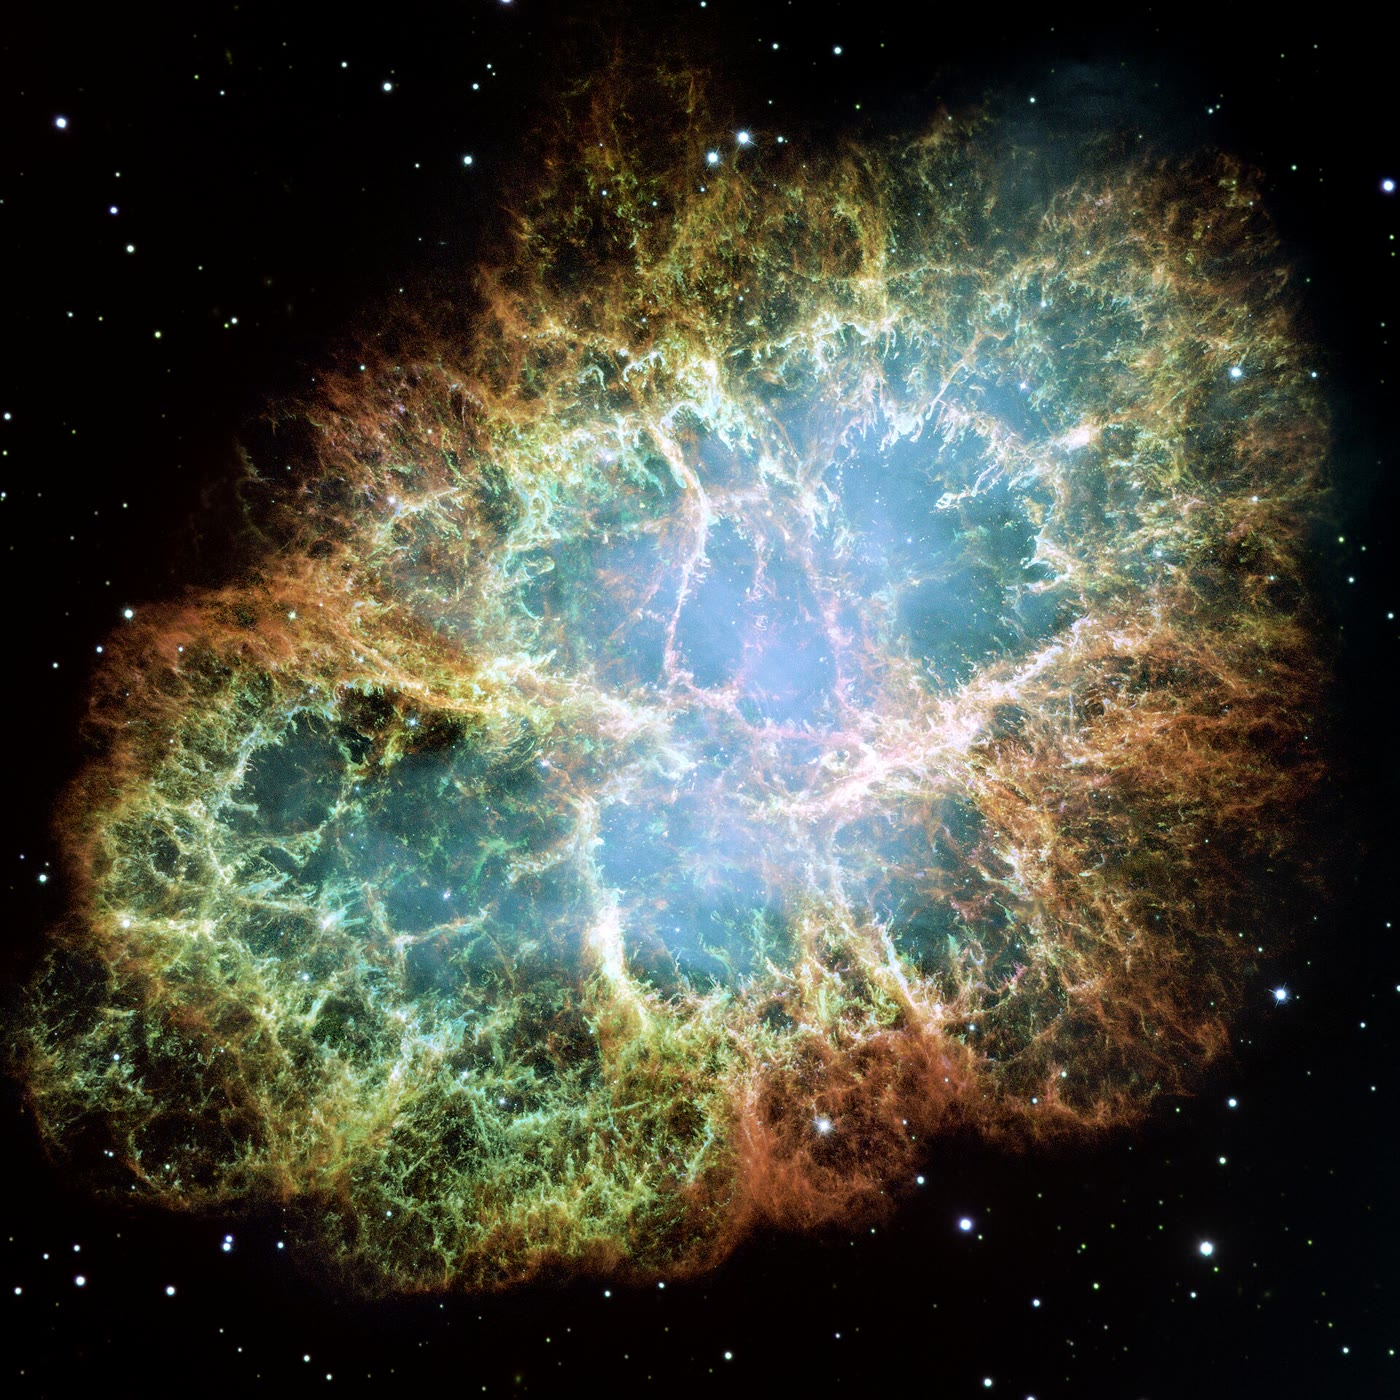
\includegraphics[width=0.5\linewidth]{images/book5/b3-crab-nebula.jpg}
\par\smallskip{\small क्रैब नेबुला, 24 हबल स्पेस टेलीस्कोप
उद्भासनों का मोज़ेक: उस तारे के फैलते अवशेष, जिसका विस्फोट
जापानी और चीनी खगोलविदों ने 1054 में अभिलेखित किया था। नारंगी तंतु
तारे की चिथड़ों जैसी बाहरी परतें हैं, मुख्यतः हाइड्रोजन; भीतर की नीली
आभा उन इलेक्ट्रॉनों से आती है जो केंद्र के न्यूट्रॉन तारे की चुंबकीय क्षेत्र
रेखाओं के चारों ओर सर्पिल गति करते हैं; यह न्यूट्रॉन तारा, जो प्रति
सेकंड तीस बार घूमता है। तंतुओं की गैस, जो तारे का बनाया पदार्थ ढोती है,
अंतरतारकीय माध्यम में मिल जाती है। NASA, ESA, J.~Hester और A.~Loll, सार्वजनिक
डोमेन।}\label{fig:b3:origin-of-elements:crab}
\end{omfigure}
% ledger: photo:b3-crab-nebula

\section{न्यूट्रॉन प्रग्रहण}\label{sec:b3:origin-of-elements:neutrons}

न्यूट्रॉन पर कोई विद्युत आवेश नहीं होता, और वह किसी नाभिक से प्रतिकर्षित नहीं होता:
धीमा न्यूट्रॉन भी उसमें प्रवेश करता है, और नाभिक, जो एक द्रव्यमान इकाई भारी हो जाता है,
बंधन ऊर्जा गामा किरण के रूप में छोड़ देता है। बार-बार प्रग्रहण से उसी तत्त्व के भारी
समस्थानिक बनते हैं, जब तक कोई अस्थिर न हो जाए; तब वह क्षय होता है,
प्रायः बीटा-ऋण क्षय से अगले तत्त्व में बदलता है, जो अपनी बारी में
प्रग्रहण करता है। कौन-से नाभिक बनते हैं, यह एक तुलना पर निर्भर है:
दो प्रग्रहणों के बीच का समय, उस मार्ग में मिलने वाले अस्थिर नाभिकों की
अर्ध-आयु से तुलना।

\begin{definition}[न्यूट्रॉन प्रग्रहण; s प्रक्रम; r प्रक्रम]\label{def:b3:origin-of-elements:s-process}
\emph{न्यूट्रॉन प्रग्रहण}\index{न्यूट्रॉन प्रग्रहण} किसी नाभिक द्वारा एक
मुक्त न्यूट्रॉन का अवशोषण है: $(Z, A) + \mathrm{n} \to (Z, A+1) + \gamma$।
\emph{s प्रक्रम}\index{s प्रक्रम} (धीमा) में प्रग्रहण
अधिकांश बीटा क्षयों से धीमे होते हैं: एक ही नाभिक पर दो प्रग्रहणों के बीच का
समय सैकड़ों से हज़ारों वर्ष है, इसलिए अस्थिर नाभिक प्रायः क्षय हो जाता है,
इससे पहले कि वह प्रग्रहण कर सके, और प्रग्रहणों तथा क्षयों की शृंखला
स्थायित्व की घाटी का अनुसरण करती है। इसके विपरीत
\emph{r प्रक्रम}\index{r प्रक्रम} (तीव्र) में न्यूट्रॉन घनत्व
इतना अधिक होता है कि प्रग्रहण क्षयों से कहीं तेज़ होते हैं: नाभिक
अत्यधिक न्यूट्रॉन-समृद्ध समस्थानिकों तक, स्थायित्व से दूर, कुछ
सेकंडों में धकेल दिए जाते हैं, और न्यूट्रॉन चुकते ही स्थायित्व की ओर क्षय होकर लौट आते हैं।
\end{definition}
% ledger: cowan21:timescales, cowan21:rprocess, kaeppeler11:overview

दोनों प्रक्रम भिन्न नाभिकों तक पहुँचते हैं, और नाभिकों का चार्ट
बताता है कि वे कौन-से हैं। नीचे की आकृति उसकी एक पट्टी दिखाती है, कैडमियम से
बेरियम तक। \omterm{def:b3:origin-of-elements:s-process}{s प्रक्रम} उसे स्थायित्व की घाटी के अनुदिश चढ़ता है: किसी तत्त्व की
पंक्ति में तब तक चलता है जब तक समस्थानिक स्थायी हैं, फिर एक बीटा क्षय से
एक पंक्ति ऊपर चढ़ता है। \omterm{def:b3:origin-of-elements:s-process}{r प्रक्रम} न्यूट्रॉन-समृद्ध ओर से आता है, नीचे दाईं ओर से:
हर अत्यधिक न्यूट्रॉन-समृद्ध नाभिक अपनी समदाब रेखा के अनुदिश क्रमिक बीटा-ऋण क्षयों से क्षय होता है,
द्रव्यमान संख्या बनाए रखते हुए, और पहले जिस स्थायी नाभिक तक पहुँचता है,
वहीं रुक जाता है। जिस स्थायी नाभिक की कम $Z$ वाली कोई स्थायी समदाब रेखा हो,
वह \omterm{def:b3:origin-of-elements:s-process}{r प्रक्रम} से \emph{परिरक्षित} होता है: $^{122}\mathrm{Te}$
$^{122}\mathrm{Sn}$ के पीछे है, $^{123}\mathrm{Te}$ $^{123}\mathrm{Sb}$ के पीछे,
और $^{124}\mathrm{Te}$ $^{124}\mathrm{Sn}$ के पीछे है।
ये तीनों केवल \omterm{def:b3:origin-of-elements:s-process}{s प्रक्रम} से बन सकते हैं: ये
\emph{केवल-s} हैं। इसके विपरीत, $^{128}\mathrm{Te}$ और $^{130}\mathrm{Te}$
s मार्ग से परे स्थित हैं, जिससे टेल्यूरियम $^{127}\mathrm{Te}$ पर रह जाता है,
जिसकी अर्ध-आयु \qty{9.35}{h} है: ये केवल-r हैं।
% ledger: kaeppeler11:overview, data:b5-iaea-gs, data:b5-sigman

\begin{omfigure}
\centering
\begin{tikzpicture}
\begin{axis}[x=0.62cm, y=0.7cm, xmin=61.4, xmax=84.6, ymin=47.4, ymax=56.6,
  xlabel={न्यूट्रॉन संख्या $N$}, ylabel={},
  xtick={62,64,...,84}, ytick={48,...,56},
  yticklabels={Cd 48, In 49, Sn 50, Sb 51, Te 52, I 53, Xe 54, Cs 55, Ba 56},
  tick label style={font=\scriptsize}, label style={font=\small},
  axis line style={black!40}, clip=false,
  scatter/classes={0={mark=square*, mark size=6.5pt, blue!45},
    1={mark=square*, mark size=6.5pt, black!18},
    2={mark=square*, mark size=6.5pt, red!40},
    3={mark=square*, mark size=6.5pt, orange!45}}]
\addplot[only marks, mark=square, mark size=6.5pt, black!45, thin,
  restrict x to domain=61:85]
  table[x=N, y=Z] {figdata/out/bachelor-3-neutron_capture-unstable.dat};
\addplot[scatter, only marks, scatter src=explicit symbolic,
  restrict x to domain=61:85]
  table[x=N, y=Z, meta=cls] {figdata/out/bachelor-3-neutron_capture-chart.dat};
\addplot[only marks, mark=none, nodes near coords={\massnum},
  restrict x to domain=61:85,
  visualization depends on={value \thisrow{A} \as \massnum},
  nodes near coords align={center}, every node near coord/.append style={font=\tiny}]
  table[x=N, y=Z] {figdata/out/bachelor-3-neutron_capture-chart.dat};
\addplot[only marks, mark=none, nodes near coords={\massnum}, restrict x to domain=61:85,
  visualization depends on={value \thisrow{A} \as \massnum},
  nodes near coords align={center}, every node near coord/.append style={font=\tiny, black!55}]
  table[x=N, y=Z] {figdata/out/bachelor-3-neutron_capture-unstable.dat};
\addplot[quiver={u=0.48*\thisrow{dN}, v=0.48*\thisrow{dZ}}, -{Stealth[length=3pt]},
  blue!60!black, semithick, restrict x to domain=61:85]
  table[x expr=\thisrow{N0}+0.26*\thisrow{dN}, y expr=\thisrow{Z0}+0.26*\thisrow{dZ}]
  {figdata/out/bachelor-3-neutron_capture-path.dat};
\begin{scope}[red!70!black, dashed, -{Stealth[length=4pt]}, thick]
\draw (axis cs:79.1,48.9) -- (axis cs:76.4,51.6);
\draw (axis cs:81.1,48.9) -- (axis cs:78.4,51.6);
\draw (axis cs:83.1,50.9) -- (axis cs:80.4,53.6);
\end{scope}
\node[font=\scriptsize, red!70!black, anchor=south east, align=right] at (axis cs:84.5,47.5)
  {r प्रक्रम क्षय\\[-1pt]समदाब रेखाओं के अनुदिश};
\end{axis}
\end{tikzpicture}
\par\smallskip{\small नाभिकों के चार्ट की एक पट्टी, कैडमियम से
बेरियम तक, न्यूट्रॉन संख्याएँ 62 से 84। रंगीन वर्ग प्रकृति में पाए गए नाभिक हैं, जिन पर
उनकी द्रव्यमान संख्या अंकित है: नीला, केवल-s; धूसर, दोनों प्रक्रमों से बना; लाल,
केवल-r; नारंगी, \omterm{def:b3:origin-of-elements:p-process}{p नाभिक}, जिन तक दोनों में से कोई नहीं पहुँचता। खुले वर्ग वे
अस्थिर नाभिक हैं जिनसे \omterm{def:b3:origin-of-elements:s-process}{s प्रक्रम} गुज़रता है। नीले तीर: s मार्ग,
प्रग्रहण दाईं ओर, बीटा क्षय तिरछे ऊपर और बाईं ओर (
$^{134}\mathrm{Cs}$ और $^{135}\mathrm{Cs}$ पर मार्ग बँट जाता है)। बिंदीदार लाल
तीर: \omterm{def:b3:origin-of-elements:s-process}{r प्रक्रम} की तीन क्षय-शृंखलाएँ, जो
$^{128}\mathrm{Te}$, $^{130}\mathrm{Te}$ और $^{134}\mathrm{Xe}$ पर समाप्त होती हैं। वर्गीकरण
प्रकृति में पाए गए समस्थानिकों से परिकलित हैं (Asplund,
Amarsi और Grevesse, 2021) और अर्ध-आयु तथा क्षय विधाएँ
IAEA के नाभिक-चार्ट से।}\label{fig:b3:origin-of-elements:chart}
\end{omfigure}
% ledger: data:b5-sigman, data:b5-iaea-gs, data:b5-asplund21, kaeppeler11:branchings

तीसरा समूह, नारंगी वर्ग, किसी भी प्रक्रम से नहीं पहुँचता:
प्रोटॉन-समृद्ध समस्थानिक, जैसे $^{112}\mathrm{Sn}$, $^{120}\mathrm{Te}$
या $^{124}\mathrm{Xe}$।

\begin{definition}[p नाभिक]\label{def:b3:origin-of-elements:p-process}
\emph{p नाभिक}\index{p नाभिक} वे स्थायी समस्थानिक हैं जो स्थायित्व-घाटी के प्रोटॉन-समृद्ध पक्ष पर,
लौह-शिखर के आगे स्थित हैं और जिन्हें न \omterm{def:b3:origin-of-elements:s-process}{s प्रक्रम} और न \omterm{def:b3:origin-of-elements:s-process}{r प्रक्रम} बना सकता है:
वे \omterm{def:b3:origin-of-elements:s-process}{r प्रक्रम} से निम्न $Z$ वाले एक स्थायी समदाब नाभिक द्वारा ढके रहते हैं
और s पथ से हटकर स्थित हैं। इन्हें एक अलग p प्रक्रम का परिणाम माना जाता है,
जो संभवतः अधिनवतारा विस्फोटों में होता है, और
कुछ अपवादों को छोड़कर इनकी प्रचुरता पड़ोसी s और r समस्थानिकों से
कहीं कम होती है।
\end{definition}
% ledger: kaeppeler11:overview

चार्ट पढ़ने वाला नियम, जब उसे ज़िंक से आगे के प्रोटो-सौर सारणी के सभी 287 नाभिकों पर लगाया जाता है,
तो 30 केवल-s नाभिक, 29 केवल-r नाभिक
और 36 \omterm{def:b3:origin-of-elements:p-process}{p नाभिक} पाए जाते हैं। इन p नाभिकों में से एक, $^{176}\mathrm{Hf}$, वास्तव में
\omterm{def:b3:origin-of-elements:s-process}{s प्रक्रम} द्वारा एक दीर्घजीवी उत्तेजित अवस्था से होकर पहुँचता है,
$^{176}\mathrm{Lu}$ की उस अवस्था जिसे सरल नियम नज़रअंदाज़ कर देता है;
बाकी 35 साहित्य के \omterm{def:b3:origin-of-elements:p-process}{p नाभिक} हैं।
% ledger: data:b5-sigman, kaeppeler11:branchings

\omterm{def:b3:origin-of-elements:s-process}{s प्रक्रम} का परिमाणात्मक अनुसरण किया जा सकता है, क्योंकि इसके नाभिक
स्थायित्व के निकट होते हैं और उनके प्रग्रहण अनुप्रस्थ-काट मापे जा सकते हैं।
किसी तारकीय प्लाज़्मा में, तापमान $T$ पर, न्यूट्रॉन ऊष्मीकृत होते हैं, और
महत्त्वपूर्ण वह अनुप्रस्थ-काट है जो उनके मैक्सवेल-बोल्ट्ज़मान
वितरण पर औसत लिया गया हो, $\langle\sigma\rangle$, जिसे एक ऊष्मीय ऊर्जा
$kT = \qty{30}{keV}$ के लिए दिया जाता है।
% ledger: kaeppeler11:classical

\begin{proposition}[$\sigma N$ संबंध]\label{prop:b3:origin-of-elements:sigma-n}
\index{sigma N relation@$\sigma N$ संबंध}
s पथ के एक ऐसे खंड पर, जहाँ हर नाभिक स्थायी हो और
न्यूट्रॉन घनत्व $n_\mathrm{n}$ तथा तापमान स्थिर हों, मान लीजिए $N_A$ द्रव्यमान-संख्या $A$ वाले नाभिक की प्रचुरता
और $\langle\sigma\rangle_A$ उसका औसत अनुप्रस्थ-काट हो।
यदि न्यूट्रॉन प्रवाह स्थायी अवस्था तक पहुँच चुका है,
तो
\[
\langle\sigma\rangle_{A-1} N_{A-1} = \langle\sigma\rangle_A N_A ,
\]
इसलिए गुणनफल $\sigma N$ खंड के
हर नाभिक के लिए समान रहता है।
\end{proposition}

\begin{proof}
द्रव्यमान $A$ वाला नाभिक न्यूट्रॉन इस दर से ग्रहण करता है
$\lambda_A = n_\mathrm{n}\langle\sigma\rangle_A v_T$ प्रति नाभिक, जहाँ
$v_T$ न्यूट्रॉनों की माध्य तापीय चाल है। यह $A - 1$ पर होने वाले प्रग्रहणों से बनता है
और स्वयं पर होने वाले प्रग्रहणों से नष्ट होता है, इसलिए
$\mathrm{d}N_A/\mathrm{d}t = n_\mathrm{n} v_T\,(\langle\sigma\rangle_{A-1}
N_{A-1} - \langle\sigma\rangle_A N_A)$ स्थायी अवस्था में अवकलज
शून्य हो जाता है, और यही संबंध है। जिस नाभिक का अनुप्रस्थ-काट बड़ा हो
वह शीघ्र आगे बढ़ जाता है और दुर्लभ रहता है; जिसका अनुप्रस्थ-काट छोटा हो
वह जमा हो जाता है।
\end{proof}
% ledger: kaeppeler11:classical

केवल-s टेल्यूरियम के तीन समस्थानिक इसकी जाँच करते हैं। इनकी प्रोटो-सौर
प्रचुरताएँ प्रति दस लाख सिलिकॉन परमाणुओं पर \num{0.1067}, \num{0.0373} और \num{0.1984} परमाणु हैं, और
उनके अनुप्रस्थ-काट \num{295}, \num{832} और \qty{155}{mb} हैं:
गुणनफल \num{31.5}, \num{31.0} और
\qty{30.8}{mb} हैं, तीन प्रतिशत के भीतर समान हैं,
यद्यपि प्रचुरताएँ पाँच गुना भिन्न हैं। एक न्यूट्रॉन जादुई संख्या के पार यह संबंध
टूट जाता है: $N = 50$, $82$ या $126$ वाले नाभिक इतने दृढ़ता से बंधे होते हैं कि
वे कम ग्रहण करते हैं: $\langle\sigma\rangle = \qty{4.0}{mb}$ है $^{138}\mathrm{Ba}$ के लिए,
जबकि $^{136}\mathrm{Ba}$ के लिए \qty{61.2}{mb} है, और
वे अवरोध का काम करते हैं। नीचे का चित्र सभी केवल-s नाभिकों का गुणनफल दिखाता है
जिसमें समतल पठार हैं, जो $A = 88$, $140$
और $208$ के निकट चरणों से अलग होते हैं।
% ledger: data:b5-sigman, data:b5-kadonis, kaeppeler11:classical

\begin{omfigure}
\centering
\begin{tikzpicture}
\begin{axis}[width=0.95\linewidth, height=7.4cm, xmin=60, xmax=212,
  ymode=log, ymin=1, ymax=5000, xlabel={द्रव्यमान-संख्या $A$},
  ylabel={$\langle\sigma\rangle N$ (mb, प्रति $10^6$ Si परमाणु)},
  tick label style={font=\scriptsize}, label style={font=\small},
  legend style={font=\scriptsize, at={(0.5,-0.17)}, anchor=north,
    legend columns=2, draw=none, cells={anchor=west},
    /tikz/every even column/.append style={column sep=1em}}]
\draw[black!35, dotted, thick] (axis cs:88,1) -- (axis cs:88,5000);
\draw[black!35, dotted, thick] (axis cs:139,1) -- (axis cs:139,5000);
\draw[black!35, dotted, thick] (axis cs:208,1) -- (axis cs:208,5000);
\addplot[blue!70!black, thick, const plot]
  table[x=A, y=sigN_model] {figdata/out/bachelor-3-neutron_capture-fitted.dat};
\addlegendentry{$A > 90$ के लिए फ़िट किया गया क्लासिकल मॉडल}
\addplot[only marks, mark=*, mark size=1.7pt, red!70!black]
  table[x=A, y=sigN] {figdata/out/bachelor-3-neutron_capture-sigman.dat};
\addlegendentry{केवल-s नाभिक}
\begin{scope}[font=\scriptsize]
\node[anchor=south west] at (axis cs:88.5,1.1) {$N = 50$};
\node[anchor=south west] at (axis cs:139.5,1.1) {$N = 82$};
\node[anchor=south east] at (axis cs:207.5,1.1) {$N = 126$};
\node[anchor=south] at (axis cs:123,38) {Te};
\node[anchor=south] at (axis cs:135,33) {Ba};
\node[anchor=north] at (axis cs:149,6.6) {Sm};
\node[anchor=west] at (axis cs:177,1.79) {Lu};
\node[anchor=west] at (axis cs:71,2326) {Ge};
\node[anchor=west] at (axis cs:83,428) {Kr};
\end{scope}
\end{axis}
\end{tikzpicture}
\par\smallskip{\small न्यूट्रॉन-ग्रहण अनुप्रस्थ-काट,
\qty{30}{keV} पर (KADoNiS) और प्रोटो-सौर प्रचुरता (Asplund,
Amarsi और Grevesse, 2021) के लिए 30 केवल-s नाभिक। जादुई
न्यूट्रॉन संख्याओं (बिंदीदार रेखाएँ) के बीच यह लगभग स्थिर है; हर एक पर प्रवाह
अवरुद्ध होता है और गुणनफल गिर जाता है। रेखा \omterm{def:b3:origin-of-elements:s-process}{s प्रक्रम} का क्लासिकल मॉडल है,
जो यहाँ $A = 90$ से भारी नाभिकों पर फ़िट किया गया है। हल्के
नाभिकों को एक दूसरा, दुर्बल घटक चाहिए, जो
विशाल तारों में बनता है।}\label{fig:b3:origin-of-elements:sigma-n}
\end{omfigure}
% ledger: data:b5-sigman, data:b5-kadonis, data:b5-asplund21, kaeppeler11:classical

चित्र की रेखा \omterm{def:b3:origin-of-elements:s-process}{s प्रक्रम} का क्लासिकल मॉडल है: लोहे-56 का एक छोटा भाग
$G$ न्यूट्रॉनों के संपर्क में आता है, और उद्भासन माध्य
$\tau_0$ के चारों ओर घातांकीय रूप से बिखरे होते हैं, और प्रवाह को
मापे गए अनुप्रस्थ-काटों के साथ नाभिक-दर-नाभिक अनुसरित किया जाता है। इसका फ़िट 22 केवल-s
नाभिकों पर, जो $A = 90$ से भारी हैं (छोड़े गए $^{176}\mathrm{Lu}$, जो
क्षय होता है, और $^{187}\mathrm{Os}$, जिसे
$^{187}\mathrm{Re}$ के क्षय से पोषण मिलता है), $\tau_0 = \qty{0.31}{mb^{-1}}$ और
सौर लोहे-56 का $G = \qty{0.054}{\percent}$ प्राप्त होता है, जो विस्तृत विश्लेषणों के
\qty{0.04}{\percent} के निकट है, जिनमें प्रत्येक बीज नाभिक औसतन लगभग
पंद्रह न्यूट्रॉन ग्रहण करता है। सबसे हल्के केवल-s
नाभिक, जर्मेनियम-70 और सेलेनियम-76, रेखा से काफ़ी ऊपर पड़ते हैं:
उन्हें एक दूसरा, दुर्बल घटक चाहिए, जो विशाल तारों में बनता है।
% ledger: data:b5-sigman, kaeppeler11:classical

जहाँ पथ पर किसी अस्थिर नाभिक का जीवनकाल लगभग उतना होता है जितना दो ग्रहणों के बीच का समय,
वहाँ प्रवाह बँट जाता है: उसका एक भाग क्षय होता है, और एक भाग ग्रहण करता है।
ऐसे \emph{शाखन} $^{79}\mathrm{Se}$, $^{85}\mathrm{Kr}$,
$^{134}\mathrm{Cs}$, $^{147}\mathrm{Pm}$ और $^{151}\mathrm{Sm}$ पर होते हैं, और अन्य कई पर भी।
शाखन से प्रवाह का एक भाग किसी नाभिक को लाँघ सकता है: सैमेरियम के दो केवल-s समस्थानिकों में से
$^{150}\mathrm{Sm}$ को पूरा प्रवाह मिलता है, और $^{148}\mathrm{Sm}$ को केवल वह भाग
जो द्रव्यमान 147 के शाखन से बचकर निकला, और उनके $\sigma N$ का अनुपात,
\num{0.87}, उस भाग को मापता है।
चूँकि वह भाग न्यूट्रॉन घनत्व और तापमान पर निर्भर है, इसलिए शाखन
उन तारों के तापमापी और घनत्वमापी हैं,
जहाँ \omterm{def:b3:origin-of-elements:s-process}{s प्रक्रम} चला।
% ledger: kaeppeler11:branchings, kaeppeler11:pairs, data:b5-sigman

\begin{inthelab}[ग्रहण अनुप्रस्थ-काट का मापन]
\omterm{def:b3:origin-of-elements:s-process}{s प्रक्रम} को आवश्यक औसत अनुप्रस्थ-काटों को मापने के लिए भौतिकीविद्
एक त्वरक पर तारकीय न्यूट्रॉन स्पेक्ट्रम का पुनरुत्पादन करते हैं।
लिथियम लक्ष्य से टकराते प्रोटॉन अभिक्रिया द्वारा न्यूट्रॉन बनाते हैं:
$^{7}\mathrm{Li}(\mathrm{p},\mathrm{n})^{7}\mathrm{Be}$, जिसका स्पेक्ट्रम
$kT = \qty{25}{keV}$ पर ऊष्मीय स्पेक्ट्रम की नक़ल करता है, जो लाल दानव के
हीलियम-कोश फ़्लैश के \qty{23}{keV} के निकट है। नमूना लक्ष्य से
बिल्कुल सटा होता है, सबसे प्रबल अभिवाह में, और विकिरण के बाद
नव-निर्मित रेडियोधर्मी नाभिकों की गामा-किरणें गिनी जाती हैं:
यह सक्रियण विधि एक माइक्रोग्राम से कम के नमूनों के साथ काम करती है।
जहाँ उत्पाद स्थायी है, न्यूट्रॉन स्पंदों में भेजे जाते हैं और एक उड़ान-पथ पर
उनका समय मापा जाता है ताकि उनकी ऊर्जा ज्ञात हो, और नमूने के चारों ओर
बेरियम फ़्लोराइड क्रिस्टलों का एक गोला प्रत्येक ग्रहण की गामा-किरण
कैस्केड अंकित करता है।
\end{inthelab}
% ledger: kaeppeler11:lab

\begin{history}[लाल दानवों में टेक्नीशियम]
1952 में P.~W.~मेरिल ने स्पेक्ट्रल प्रकार S के लाल दानवों के स्पेक्ट्रम में
टेक्नीशियम की रेखाएँ पाईं। टेक्नीशियम का कोई स्थायी समस्थानिक नहीं है; \omterm{def:b3:origin-of-elements:s-process}{s प्रक्रम} द्वारा बना
समस्थानिक $^{99}\mathrm{Tc}$ की अर्ध-आयु
\num{211000} वर्ष है, जो उन तारों द्वारा जी गई अवधियों से
कहीं कम है। टेक्नीशियम का तारों के भीतर बना होना आवश्यक था, और
हाल में ही। यह तारों द्वारा तत्त्व बनाने का पहला प्रत्यक्ष प्रमाण था।
1957 में E.~M. और G.~R.~बर्बिज, W.~A.~फ़ाउलर और F.~हॉयल, तथा
स्वतंत्र रूप से A.~G.~W.~कैमरन ने \omterm{def:b3:origin-of-elements:s-process}{s प्रक्रम} के क्लासिकल
मॉडल का सूत्रण किया।
\end{history}
% ledger: kaeppeler11:overview, data:b5-iaea-gs

\omterm{def:b3:origin-of-elements:s-process}{r प्रक्रम} अपने स्वयं के शिखर छोड़ता है। इसका पथ न्यूट्रॉन-ड्रिप रेखा के
निकट चलता है, यानी वह सीमा जिसके आगे कोई नाभिक एक और न्यूट्रॉन नहीं रख सकता,
और प्रवाह बंद न्यूट्रॉन कोशों वाले नाभिकों पर रुकता है: $N = 50$, $82$ और
$126$, जब तक वे बीटा-क्षय नहीं करते। ये प्रतीक्षा-बिंदु पदार्थ जमा करते हैं;
स्थायित्व तक के अंतिम क्षयों के बाद ये ढेर कुछ इकाई कम द्रव्यमान संख्याओं पर
उन्हीं जादुई संख्याओं वाले s-प्रक्रम शिखरों की तुलना में पड़ते हैं, जो स्थायी नाभिकों से बने हैं:
$A = 130$ (टेल्यूरियम और ज़ीनॉन) के निकट और $A = 195$ (प्लैटिनम),
बनाम बेरियम और सीसा के s शिखरों के लिए $A = 138$ और $208$।
प्रचुरता वक्र दोनों समुच्चयों के शिखर
साथ-साथ दिखाता है। \omterm{def:b3:origin-of-elements:s-process}{r प्रक्रम} भारी तत्त्वों का लगभग आधा
बनाता है, और \omterm{def:b3:origin-of-elements:s-process}{s प्रक्रम} दूसरा आधा।
% ledger: cowan21:rprocess, kaeppeler11:overview, kaeppeler11:classical

\section{प्रक्रम कहाँ चलते हैं}\label{sec:b3:origin-of-elements:sites}

मुख्य \omterm{def:b3:origin-of-elements:s-process}{s प्रक्रम} लगभग तीन सौर द्रव्यमान तक की लाल दानवों में चलता है, उनके जीवन के
अंतिम चरण के निकट, असिम्प्टोटिक-जाइंट-शाखा तारों के रूप में। उनके केंद्रों के चारों
ओर एक कोश में हीलियम दहन की लपटों के बीच, कार्बन-13 से समृद्ध एक पतली परत
बनती है; लगभग \qty{9e7}{K} पर अभिक्रिया
$^{13}\mathrm{C}(\alpha,\mathrm{n})^{16}\mathrm{O}$ न्यूट्रॉन मुक्त करती है
कुछ दस हज़ार वर्षों तक, घनत्व $10^6$ से
\num{e8}\text{ न्यूट्रॉन}\,\unit{cm^{-3}} तक। स्वयं लपटों के दौरान, \qty{2.5e8}{K} से
ऊपर, $^{22}\mathrm{Ne}(\alpha,\mathrm{n})^{25}\mathrm{Mg}$ अभिक्रिया
\qty{e10}{cm^{-3}} तक घनत्व पर कुछ वर्षों का एक विस्फोट देती है। उत्पाद
सतह तक ऊपर लाए जाते हैं, जहाँ टेक्नीशियम देखा जाता है, और तारे की
पवन में उड़ा दिए जाते हैं। दुर्बल \omterm{def:b3:origin-of-elements:s-process}{s प्रक्रम}, जो $A = 90$ से हल्के केवल-s नाभिक बनाता है,
विशाल तारों में उनके हीलियम और
कार्बन दहन के दौरान चलता है।
% ledger: kaeppeler11:sources, kaeppeler11:overview

कोर-पतन अधिनवतारे, जो आठ से दस सौर द्रव्यमान से ऊपर के तारों का अंत हैं,
\omterm{def:b3:origin-of-elements:alpha}{अल्फ़ा तत्त्व} और लोहे का एक भाग तारों के जन्म के तुरंत बाद लौटाते हैं, क्योंकि विशाल तारों का
जीवन छोटा होता है। टाइप Ia अधिनवतारे, जो
द्विआधारी तंत्रों में विस्फोट करने वाले श्वेत वामन हैं, अधिकांश लोहा लौटाते हैं,
पर केवल एक विलंब के बाद: श्वेत वामन को पहले आठ सौर द्रव्यमान से कम
के एक तारे से बनना पड़ता है, और फिर या तो किसी साथी से पदार्थ बटोरकर
चंद्रशेखर द्रव्यमान तक पहुँचना, जो लगभग
\qty{1.44}{M_\odot} है, या दूसरे श्वेत वामन के साथ विलय होना। \omterm{def:b3:origin-of-elements:s-process}{r प्रक्रम} को
इससे कहीं अधिक चरम स्थान चाहिए।
% ledger: matteucci21:production, matteucci21:time-delay

\begin{definition}[न्यूट्रॉन-तारा विलय; किलोनोवा]\label{def:b3:origin-of-elements:kilonova}
\emph{न्यूट्रॉन-तारा विलय}\index{न्यूट्रॉन-तारा विलय} एक निकट द्विआधारी
तंत्र में दो न्यूट्रॉन तारों का संयोजन है, जिसकी कक्षा
गुरुत्वीय तरंगों के उत्सर्जन से सिकुड़ गई है। न्यूट्रॉन-समृद्ध पदार्थ का एक भाग
बाहर फेंक दिया जाता है। \emph{किलोनोवा}\index{किलोनोवा} उस इजेक्टा की
क्षणिक दीप्ति है, जिसे ताज़े बने \omterm{def:b3:origin-of-elements:s-process}{r प्रक्रम} नाभिकों का रेडियोधर्मी क्षय तप्त करता है,
और जो कुछ दिनों तक रहती है।
\end{definition}
% ledger: cowan21:kilonova, ligo17:gw170817

17 अगस्त 2017 को गुरुत्वीय-तरंग संसूचकों ने
दो न्यूट्रॉन तारों, GW170817, के अंतर्वलन को लगभग
\qty{40}{Mpc} दूरी पर अंकित किया: दो पिंड, \num{1.17} से \qty{1.60}{M_\odot} के, कुल
\qty{2.74}{M_\odot}। एक गामा-किरण विस्फोट विलय के \qty{1.7}{s} बाद
पहुँचा। ग्यारह घंटे से कम बाद दूरबीनों को एक नया प्रकाश-बिंदु मिला,
मंदाकिनी NGC~4993 में (नीचे का चित्र)। उसकी पराबैंगनी दीप्ति
दो दिनों के भीतर फीकी पड़ गई, और दस दिनों में उसका प्रकाश लाल और अवरक्त हो गया।
उस विकास के मॉडलों को इजेक्टा के कई घटक चाहिए, जिनमें सबसे लाल
घटक लैंथेनाइडों से समृद्ध है, यानी भारी \omterm{def:b3:origin-of-elements:s-process}{r प्रक्रम} तत्त्वों से, जिनका
रेखाओं का घना वन इजेक्टा को अपारदर्शी बना देता है। कुल निष्कासित द्रव्यमान
\num{0.03} से \qty{0.08}{M_\odot} तक आँका गया है: पहला प्रत्यक्ष
प्रमाण कि \omterm{def:b3:origin-of-elements:kilonova}{न्यूट्रॉन-तारा विलय} \omterm{def:b3:origin-of-elements:s-process}{r प्रक्रम} तत्त्व बनाते हैं।
% ledger: ligo17:gw170817, mma17:kilonova, cowan21:kilonova

\begin{omfigure}
\centering
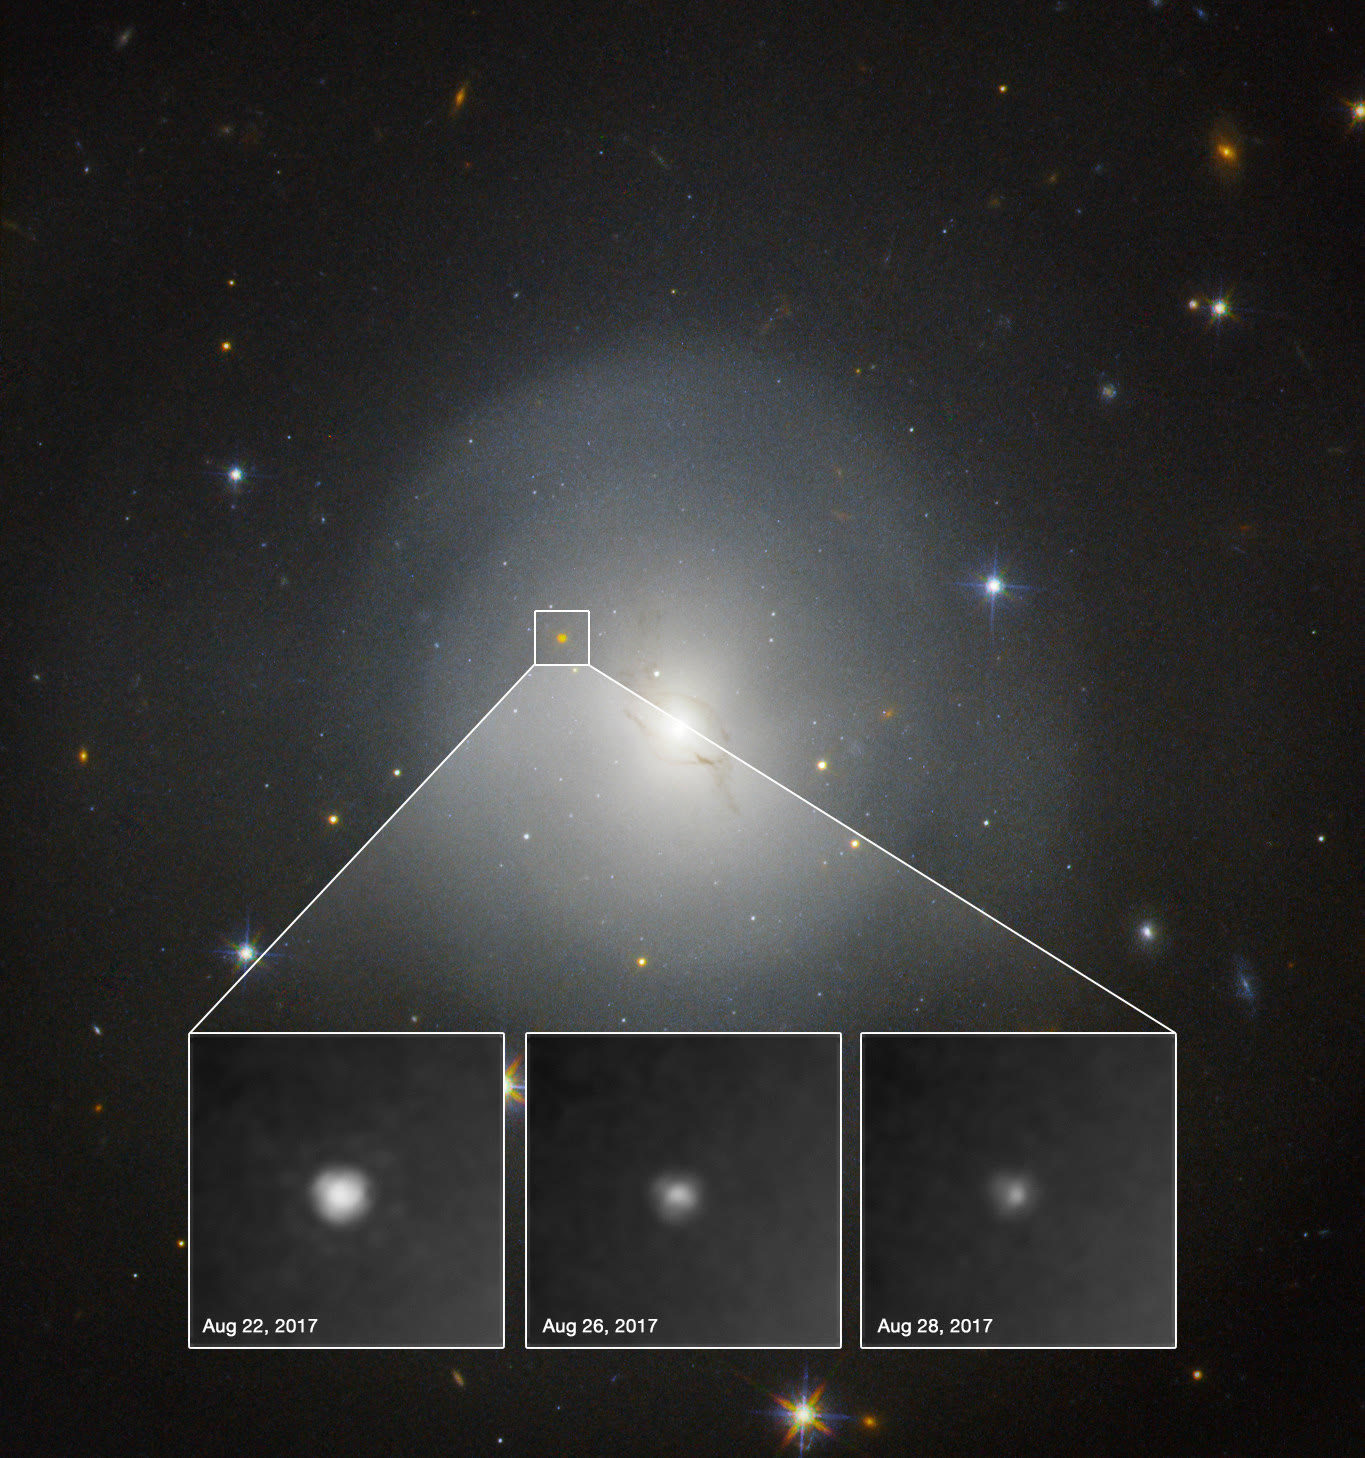
\includegraphics[width=0.55\linewidth]{images/book5/b3-kilonova.jpg}
\par\smallskip{\small मंदाकिनी NGC~4993 का चित्र, जिसे हबल
स्पेस टेलीस्कोप ने दो न्यूट्रॉन तारों के विलय के बाद खींचा, जिनका
विलय गुरुत्वाकर्षी तरंगों में 17 अगस्त 2017 को पहचाना गया था। घेरा \omterm{def:b3:origin-of-elements:kilonova}{किलोनोवा} को
चिह्नित करता है; 22, 26 और 28 अगस्त को लिए गए इनसेट में वह छह दिनों में फीका पड़ता दिखता है।
NASA और ESA (A.~J.~Levan, N.~R.~Tanvir, A.~Fruchter और O.~Fox), CC
BY~4.0.}\label{fig:b3:origin-of-elements:kilonova}
\end{omfigure}
% ledger: photo:b3-kilonova

\begin{dated}{2021}
क्या \omterm{def:b3:origin-of-elements:kilonova}{न्यूट्रॉन-तारा विलय} आकाशगंगा के अधिकांश \omterm{def:b3:origin-of-elements:s-process}{r प्रक्रम}
तत्त्व बनाते हैं, यह अभी तय नहीं है। विलय अपनी द्विआधारी कक्षाओं के क्षय की
प्रतीक्षा करते हैं, और आकाशगंगा के विकास के ऐसे मॉडल, जिनमें विलय ही एकमात्र स्रोत हैं,
\omterm{def:b3:origin-of-elements:s-process}{r प्रक्रम} तत्त्वों को इतनी देर से बनाते हैं कि वे उसकी व्याख्या नहीं कर पाते
जो सबसे पुराने, सबसे कम \omterm{def:b3:origin-of-elements:metallicity}{धात्विकता} वाले तारों में देखा जाता है। क्रोड-पतन अधिनवतारा के कुछ दुर्लभ प्रकार,
जिनमें तीव्र घूर्णन और प्रबल चुंबकीय क्षेत्र हैं, तथा अति विशाल तारों का पतन
अन्य संभावित स्रोत हैं; आकाशगंगा का एक मॉडल देखे गए यूरोपियम की व्याख्या
तभी करता है यदि लगभग तीन प्रतिशत हाइपरनोवा, जिनका द्रव्यमान
25 से \qty{50}{M_\odot} के बीच है, चुंबकीय रूप से
संचालित प्रकार के हों।
\end{dated}
% ledger: kobayashi20:origins, cowan21:rprocess

\section{आकाशगंगा का रासायनिक विकास}\label{sec:b3:origin-of-elements:gce}

हर पीढ़ी के तारे अपनी बनाई कुछ सामग्री गैस में लौटा देते हैं, और
अगली पीढ़ी उसी समृद्ध गैस से बनती है। किसी तारे का संघटन
इसलिए उसके जन्म के समय की गैस का संघटन दर्ज करता है, और
आयु के अनुसार छाँटे गए किसी मंदाकिनी के तारे उसका इतिहास दर्ज करते हैं।

\begin{definition}[मंदाकिनीय रासायनिक विकास]\label{def:b3:origin-of-elements:gce}
\emph{मंदाकिनीय रासायनिक विकास}\index{मंदाकिनीय रासायनिक विकास}
किसी मंदाकिनी की गैस और तारों के संघटन में समय के साथ होने वाला परिवर्तन है, जो
तारा-निर्माण, \omterm{def:b3:origin-of-elements:yield}{तारकीय लब्धि}, तारों के जीवनकाल और मंदाकिनी में आने
या उससे बाहर निकाली जाने वाली गैस के संयुक्त प्रभाव से होता है;
और उस परिवर्तन का अध्ययन उन मॉडलों द्वारा किया जाता है
जिनकी तुलना ज्ञात आयु के तारों की प्रचुरता से की जाती है।
\end{definition}
% ledger: matteucci21:simple

सबसे सरल मॉडल मंदाकिनी के एक क्षेत्र को भली-भाँति मिश्रित गैस की एक पेटिका मानता है,
जो धीरे-धीरे तारों में बदलती है। मान लीजिए $s$ लंबे-जीवी तारों और तारकीय अवशेषों में
बंद द्रव्यमान है, $M_\mathrm{g}$ गैस का द्रव्यमान, और
$M = M_\mathrm{g} + s$ कुल द्रव्यमान। \emph{प्रति तारकीय
पीढ़ी लब्धि} $y$ वह नई धातुओं का द्रव्यमान है जिसे तारों की एक पीढ़ी
उसके द्वारा बंद किए गए प्रति एकक द्रव्यमान पर गैस में लौटाती है।
% ledger: matteucci21:yield

\begin{theorem}[बंद-पेटिका मॉडल]\label{thm:b3:origin-of-elements:closed-box}
\index{बंद-पेटिका मॉडल}
विचार कीजिए एक ऐसा क्षेत्र जो अपने परिवेश के साथ कोई गैस नहीं बदलता, शुद्ध,
धातु-रहित गैस के रूप में आरंभ होता है, भली-भाँति मिश्रित रहता है, और उसमें
धातु बनाने वाले तारे तुरंत मर जाते हैं, जबकि अन्य तारे सदा जीते हैं
(तात्क्षणिक पुनर्चक्रण)। तब गैस की \omterm{def:b3:origin-of-elements:metallicity}{धात्विकता} इस प्रकार है:
\[
Z = y \ln\frac{1}{\mu}, \qquad \mu = \frac{M_\mathrm{g}}{M},
\]
जहाँ $\mu$ गैस-अंश है, और
$Z$ से कम \omterm{def:b3:origin-of-elements:metallicity}{धात्विकता} के साथ बने तारों का द्रव्यमान \mbox{$M\,(1 - \mathrm{e}^{-Z/y})$} है।
\end{theorem}

\begin{proof}
जब द्रव्यमान $\mathrm{d}s$ तारों में बंद होता है, तब गैस
$\mathrm{d}s$ खो देती है, साथ में उसमें मौजूद धातुएँ $Z\,\mathrm{d}s$,
और $y\,\mathrm{d}s$ नई धातुएँ प्राप्त करती है:
तथा $\mathrm{d}M_\mathrm{g} = -\mathrm{d}s$
$\mathrm{d}(Z M_\mathrm{g}) = (y - Z)\,\mathrm{d}s$। दूसरे समीकरण का
विस्तार करने पर $M_\mathrm{g}\,\mathrm{d}Z + Z\,\mathrm{d}M_\mathrm{g} =
y\,\mathrm{d}s - Z\,\mathrm{d}s$, और $Z$ वाले पद निरस्त हो जाते हैं:
$M_\mathrm{g}\,\mathrm{d}Z = -y\,\mathrm{d}M_\mathrm{g}$। समाकलन करने पर
$M_\mathrm{g} = M$, $Z = 0$ से आरंभ करने पर $Z = y\ln(M/M_\mathrm{g})$ प्राप्त होता है। वे
तारे, जो गैस की \omterm{def:b3:origin-of-elements:metallicity}{धात्विकता} $Z$ से नीचे रहते समय बने, वही हैं
जो तब बने जब गैस $M$ से घटकर $M\mathrm{e}^{-Z/y}$ हुई, वह द्रव्यमान
$M(1 - \mathrm{e}^{-Z/y})$ है।
\end{proof}
% ledger: matteucci21:simple

यह मॉडल लंबे-जीवी तारों के धात्विकता-वितरण का पूर्वानुमान करता है।
सौर पड़ोस में गैस का पृष्ठ-घनत्व
\qty{13.7}{M_\odot.pc^{-2}} है, और तारों तथा तारकीय अवशेषों का
\qty{33.4}{M_\odot.pc^{-2}} है, इसलिए $\mu = 13.7/47.1 = 0.29$।
यदि आज की गैस में आद्य-सौर $Z = 0.0154$ है, तो लब्धि
$y = 0.0154/\ln(1/0.29) = 0.0125$ है, और अब तक बने सभी तारों में वह अंश
जिनकी $Z$ वर्तमान मान के दसवें भाग से कम है,
$[\mathrm{Fe/H}] < -1$ यदि लोहा धातुओं का अनुसरण करता है, वह
$(1 - 0.29^{0.1})/(1 - 0.29) = 0.16$ है।
% ledger: mckee15:surface, asplund21:xyz, data:b5-gce

\begin{omfigure}
\centering
\begin{tikzpicture}
\begin{axis}[width=0.95\linewidth, height=7.2cm, xmin=-1.6, xmax=0.7,
  ymin=0, ymax=1500, xlabel={$[\mathrm{Fe/H}]$},
  ylabel={प्रति \num{0.1}~डेक्स तारों की संख्या},
  tick label style={font=\scriptsize}, label style={font=\small},
  legend style={font=\scriptsize, at={(0.5,-0.17)}, anchor=north,
    legend columns=3, draw=none, cells={anchor=west},
    /tikz/every even column/.append style={column sep=1em}}]
\addplot[ybar, area legend, bar width=0.085, fill=black!25, draw=black!50, bar shift=0pt]
  table[x=feh, y=n_obs] {figdata/out/bachelor-3-chemical_evolution-mdf.dat};
\addlegendentry{F और G वामन (6670)}
\addplot[ybar, area legend, bar width=0.085, fill=blue!55, draw=blue!70!black, bar shift=0pt]
  table[x=feh, y=n_low] {figdata/out/bachelor-3-chemical_evolution-mdf.dat};
\addlegendentry{\qty{1}{M_\odot} तक (902)}
\addplot[red!75!black, very thick, const plot mark mid]
  table[x=feh, y=model] {figdata/out/bachelor-3-chemical_evolution-mdf.dat};
\addlegendentry{बंद पेटिका}
\draw[black!50, dashed] (axis cs:-1,0) -- (axis cs:-1,1500);
\node[font=\scriptsize, anchor=north west, align=left] at (axis cs:-1.57,1450)
  {बंद पेटिका: \qty{16}{\percent}\\$-1$ से नीचे;\\प्रेक्षित: \qty{0.4}{\percent}};
\end{axis}
\end{tikzpicture}
\par\smallskip{\small \omterm{def:b3:origin-of-elements:g-dwarf}{G-वामन समस्या}। स्तंभ: धात्विकताएँ
सौर पड़ोस के F और G वामनों की (जिनेवा--कोपेनहेगन
सर्वेक्षण, सर्वोत्तम-प्रकाशमिति नमूना, जिसे कासाग्रांडे और अन्य ने
2011 में पुनर्विश्लेषित किया), सभी तारे धूसर में, वे जो अधिकतम एक सौर द्रव्यमान के हैं, वे दीर्घजीवी
तारे जिन्हें मॉडल गिनता है, नीले में। रेखा: बंद
पेटिका, जो सौर पड़ोस के वर्तमान गैस-अंश के साथ है और
उतनी ही तारा-संख्या तक मापी गई है; यह किसी तारे को अपनी वर्तमान गैस से, जिसे सौर लिया गया है, अधिक
धातु-समृद्ध नहीं बनाती। पेटिका कम \omterm{def:b3:origin-of-elements:metallicity}{धात्विकता} वाले
तारों की एक लंबी पूँछ का पूर्वानुमान करती है, जो वहाँ नहीं है।}\label{fig:b3:origin-of-elements:g-dwarf}
\end{omfigure}
% ledger: data:b5-gcs, casagrande11:gcs, data:b5-gce, mckee15:surface

\begin{definition}[G-वामन समस्या]\label{def:b3:origin-of-elements:g-dwarf}
\emph{G-वामन समस्या}\index{G-वामन समस्या} सौर पड़ोस में कम \omterm{def:b3:origin-of-elements:metallicity}{धात्विकता} वाले दीर्घजीवी तारों की
कमी है, जो \omterm{thm:b3:origin-of-elements:closed-box}{बंद-पेटिका मॉडल} के अनुमान की तुलना में दिखती है:
स्पेक्ट्रल प्रकार G के दीर्घजीवी वामन तारों में से बहुत कम तारों की
\omterm{def:b3:origin-of-elements:metallicity}{धात्विकता} निम्न होती है, जितनी बंद पेटिका के मॉडल में
बनी होती।
\end{definition}
% ledger: matteucci21:simple

सर्वेक्षण नमूने के 6670 तारों में से 26 की $[\mathrm{Fe/H}] < -1$ है:
\qty{0.4}{\percent}, जबकि बंद पेटिका में यह \qty{16}{\percent} है।
अधिकतम एक सौर द्रव्यमान के 902 तारों में भी, जो सबसे उचित तुलना है,
26 तारे \qty{2.9}{\percent} बनाते हैं। इससे बचने का उपाय यह है कि
पेटिका खोली जाए: यदि सौर पड़ोस की चक्रिका कम \omterm{def:b3:origin-of-elements:metallicity}{धात्विकता} वाली गैस के
धीमे अंतर्वाह से कई अरब वर्षों में बनी है, तो आरंभिक गैस कभी
कम \omterm{def:b3:origin-of-elements:metallicity}{धात्विकता} वाले तारे बनाने के लिए प्रतीक्षारत बड़ा भंडार नहीं थी, और पूँछ
लुप्त हो जाती है। चक्रिका के वे मॉडल जो वितरण को पुनरुत्पादित करते हैं,
उनमें अंतर्वाह काल तीन से चार अरब वर्ष से अधिक चाहिए।
% ledger: data:b5-gcs, data:b5-gce, matteucci21:simple

दूसरी घड़ी दो प्रकार के तत्त्वों का अनुपात है। \omterm{def:b3:origin-of-elements:alpha}{अल्फ़ा तत्त्व}
कोर-पतन अधिनवतारों से आते हैं, तारकीय पीढ़ी के जन्म के तुरंत बाद;
लोहे का बड़ा भाग टाइप~Ia अधिनवतारों से आता है,
बहुत बाद में। पुराने प्रभामंडल तारों में, जिनकी $[\mathrm{Fe/H}] < -1$ है,
$[\alpha/\mathrm{Fe}]$ लगभग $+0.4$ होता है: ये तारे केवल कोर-पतन अधिनवतारों से
समृद्ध गैस से बने। चक्रिका के तारों में \omterm{def:b3:origin-of-elements:metallicity}{धात्विकता} बढ़ने के साथ यह
शून्य तक, यानी सौर मान तक, गिरता है, जब टाइप~Ia
अधिनवतारे अपना लोहा जोड़ते हैं। नीचे का चित्र इस
\emph{समय-विलंब} चित्र का सरलतम मॉडल दिखाता है: एक बंद पेटिका में दोनों प्रकार के
अधिनवतारे एक साथ आरंभ होते हैं, सिवाय इसके कि टाइप~Ia अधिनवतारे
पहले तारों के बाद एक निश्चित विलंब से आरंभ होते हैं।
% ledger: matteucci21:time-delay, matteucci21:production

\begin{omfigure}
\centering
\begin{tikzpicture}
\begin{axis}[width=0.8\linewidth, height=6.4cm, xmin=-2.4, xmax=0.25,
  ymin=-0.08, ymax=0.55, xlabel={$[\mathrm{Fe/H}]$},
  ylabel={$[\alpha/\mathrm{Fe}]$},
  tick label style={font=\scriptsize}, label style={font=\small}]
\addplot[black!40, dashed, domain=-2.4:0.25, samples=2] {0};
\addplot[blue!70!black, very thick]
  table[x=feh, y=afe] {figdata/out/bachelor-3-chemical_evolution-alpha.dat};
\addplot[only marks, mark=*, mark size=2pt, red!70!black] coordinates {(-1,0.4) (0,0)};
\node[font=\scriptsize, anchor=south, align=center] at (axis cs:-1.75,0.41)
  {केवल कोर-पतन अधिनवतारे};
\node[font=\scriptsize, anchor=south west, align=left] at (axis cs:-0.98,0.41)
  {टाइप Ia अधिनवतारे\\[-1pt]आरंभ};
\node[font=\scriptsize, anchor=south west] at (axis cs:0.01,0.01) {सूर्य};
\end{axis}
\end{tikzpicture}
\par\smallskip{\small एक बंद पेटिका में $[\alpha/\mathrm{Fe}]$ का दो-चरणीय मॉडल
$+0.4$ पर पठार वह अनुपात है जो कोर-पतन
अधिनवतारे बनाते हैं; टाइप~Ia अधिनवतारे, जो तब आरंभ होते हैं जब गैस
$[\mathrm{Fe/H}] = -1$ तक पहुँच जाती है, फिर स्थिर दर से लोहा जोड़ते हैं, जब तक
$[\mathrm{Fe/H}] = 0$ पर अनुपात सौर नहीं हो जाता। पठार और घुटना वे हैं
जो आकाशगंगा के तारों में दिखते हैं; बीच का आकार मॉडल का है।
सूर्य की \omterm{def:b3:origin-of-elements:metallicity}{धात्विकता} पर इस मॉडल में लोहे का \qty{60}{\percent} भाग
टाइप~Ia अधिनवतारों से आया है।}\label{fig:b3:origin-of-elements:alpha}
\end{omfigure}
% ledger: data:b5-gce, matteucci21:time-delay

प्रेक्षित प्रवृत्ति को पुनरुत्पादित करने वाले आकाशगंगा के विस्तृत मॉडल
लोहे का दो-तिहाई टाइप~Ia अधिनवतारों से और एक-तिहाई
कोर-पतन अधिनवतारों से लेते हैं, और पाते हैं कि युवा आकाशगंगा की गैस
$[\mathrm{Fe/H}] = -1$ तक लगभग एक से डेढ़ अरब
वर्षों में पहुँच गई थी। यह अनुपात एक घड़ी है: किसी दिए गए \omterm{def:b3:origin-of-elements:metallicity}{धात्विकता} पर अल्फ़ा तत्त्वों से समृद्ध समष्टि
ने अपने तारे तेज़ी से बनाए थे, इससे पहले कि
टाइप~Ia अधिनवतारे अपना लोहा जोड़ पाते। पिछले अध्याय की \omterm{def:b3:milky-way-galaxies:structure}{मोटी चक्रिका}
ऐसी ही समष्टि है: पुरानी, और उसी \omterm{def:b3:origin-of-elements:metallicity}{धात्विकता} की
पतली-चक्रिका तारों की तुलना में अल्फ़ा तत्त्वों से कुछ समृद्ध।
% ledger: matteucci21:time-delay, casagrande11:gcs

\section{सौर प्रचुरता से पृथ्वी तक}\label{sec:b3:origin-of-elements:earth}

पृथ्वी उसी पदार्थ से बनी है जिससे सूर्य बना है, पर उसके सारे
पदार्थ से नहीं। शीतलन करती नीहारिका में केवल वही तत्त्व जो
ठोस रूप में संघनित हुए, ग्रहाणुओं में एकत्र हो सकते थे; पुस्तक 4 (स्नातक वर्ष 2) उस
क्रम का अनुसरण करती है जिसमें वे संघनित होते हैं। लोहा धातु के रूप में मैग्नीशियम सिलिकेटों के
लगभग समान तापमान पर संघनित होता है, \qtyrange{1310}{1340}{K} के बीच, \qty{e-4}{bar} पर,
इसलिए चट्टानी ग्रहों ने अपने लोहे का अंश रखा, जबकि
हाइड्रोजन, हीलियम, कार्बन, नाइट्रोजन और उत्कृष्ट गैसें गैस में ही रहीं।
सौर संघटन की गैस में केवल लगभग आधा प्रतिशत द्रव्यमान
चट्टान और धातु के रूप में संघनित होता है।
% ledger: lodders:tc-table, lodders:condensates

\begin{definition}[वाष्पशीलता प्रवृत्ति]\label{def:b3:origin-of-elements:volatility}
किसी ग्रहीय पिंड की \emph{वाष्पशीलता प्रवृत्ति}\index{वाष्पशीलता प्रवृत्ति} वह ह्रास है
जो CI कॉन्ड्राइटों के सापेक्ष, और एक दुर्गलनीय तत्त्व पर सामान्यीकृत,
संघनन तापमान घटने के साथ उसकी प्रचुरताओं में होता है:
दुर्गलनीय तत्त्व अपने कॉन्ड्राइट अनुपात में रहते हैं,
जबकि मध्यम वाष्पशील तत्त्व जितने कम संघनन तापमान के होते हैं,
उतने ही अधिक घटे होते हैं।
\end{definition}

सिलिकेट पृथ्वी के लिए, पुस्तक 4 (स्नातक वर्ष 2) ने प्रवृत्ति को संघनन
तापमान के विरुद्ध खींचा। मैग्नीशियम पर सामान्यीकृत, ज़िरकोनियम
(\qty{1741}{K} पर संघनित होता है) अपने CI अनुपात का \num{1.11} गुना है,
सोडियम (\qty{958}{K}) पर \num{0.22}, पोटैशियम
(\qty{1006}{K}) पर \num{0.19}, रूबिडियम (\qty{800}{K}) पर \num{0.12}
और ज़िंक (\qty{726}{K}) पर \num{0.075}। पृथ्वी ऐसे पदार्थ से बनी जो
ग्रह के जुड़ने से पहले ही अपने मध्यम वाष्पशील तत्त्वों का कुछ भाग खो चुका था,
या अपनी वृद्धि के दौरान उन्हें खो बैठी। यहाँ तक कि CI
कॉन्ड्राइट भी सूर्य से इस प्रकार भिन्न हैं जो संघनन
तापमान का अनुसरण करता है, यद्यपि हल्के रूप में: उनके मध्यम वाष्पशील तत्त्व
लगभग \num{0.04}~\omterm{def:b3:origin-of-elements:abundance}{डेक्स} अधिक हैं, प्रकाशमंडलीय मानों से।
% ledger: lodders:tc-table, lodders:ci-table, ms95:pm-trace, asplund21:abstract

अतः इस अध्याय का अभिलेख ग्रह के भीतर तक जाता है। प्रावार के
ऑक्सीजन, मैग्नीशियम और सिलिकन विशाल तारों के \omterm{def:b3:origin-of-elements:alpha}{अल्फ़ा तत्त्व} हैं;
क्रोड का लोहा अधिकतर टाइप~Ia अधिनवतारों से आया;
थोरियम और यूरेनियम, जिनका क्षय भीतरी भाग को गरम करने में मदद करता है,
बिस्मथ के परे स्थित हैं, जहाँ केवल \omterm{def:b3:origin-of-elements:s-process}{r प्रक्रम} पहुँचता है; और पूरा मिश्रण
पृथ्वी के उसे जुटाने से पहले वाष्पशीलता के अनुसार छँट चुका था।
% ledger: matteucci21:production, matteucci21:time-delay, kaeppeler11:overview, data:b5-sigman

\section{अभ्यास}

\begin{exercise}[$\star$]\label{exo:b3:origin-of-elements:1}
सूर्य की सौर प्रचुरताएँ $\log\varepsilon(\mathrm{O}) = 8.69$,
$\log\varepsilon(\mathrm{Si}) = 7.51$, $\log\varepsilon(\mathrm{Fe}) =
7.46$, $\log\varepsilon(\mathrm{Au}) = 0.91$ और
$\log\varepsilon(\mathrm{Pb}) = 1.95$ लेकर: (क)~सूर्य में लोहे के प्रति
परमाणु पर कितने सिलिकन परमाणु और कितने ऑक्सीजन परमाणु हैं? (ख)~सोने के प्रति
परमाणु पर कितने लोहा परमाणु, और कितने सीसा परमाणु हैं?
\end{exercise}

\begin{exercise}[$\star$]\label{exo:b3:origin-of-elements:2}
(क)~सूर्य में प्रति दस लाख हाइड्रोजन परमाणुओं पर कितने लोहा परमाणु होते हैं
($\log\varepsilon(\mathrm{Fe}) = 7.46$)? (ख)~एक प्रभामंडल तारे का
$[\mathrm{Fe/H}] = -2$ है। उसमें प्रति लोहा परमाणु पर हाइड्रोजन के कितने परमाणु होते हैं?
(ग)~एक अन्य तारे में हाइड्रोजन के प्रति एक करोड़ परमाणुओं पर एक लोहा परमाणु है।
इसका $[\mathrm{Fe/H}]$ क्या है?
\end{exercise}

\begin{exercise}[$\star$]\label{exo:b3:origin-of-elements:3}
ज़ेनॉन के स्थायी समस्थानिकों की द्रव्यमान संख्याएँ 124, 126, 128, 129, 130,
131, 132, 134 और 136 हैं। उनके समभारों में से टेल्यूरियम ($Z = 52$) के
स्थायी समस्थानिक 120, 122--126, 128 और 130 हैं; आयोडीन ($Z = 53$) का केवल 127 है।
s पथ ज़ेनॉन तक $^{128}\mathrm{Xe}$ पर पहुँचता है, $^{128}\mathrm{I}$ के
क्षय से; और $^{133}\mathrm{Xe}$ पर उसे छोड़ता है, जो स्वयं क्षय होता है।
प्रत्येक ज़ेनॉन समस्थानिक को केवल-s, केवल-r, दोनों द्वारा निर्मित, या \omterm{def:b3:origin-of-elements:p-process}{p
नाभिक} के रूप में वर्गीकृत कीजिए।
\end{exercise}

\begin{exercise}[$\star$]\label{exo:b3:origin-of-elements:4}
GW170817 लगभग \qty{40}{Mpc} दूर स्थित था, और उसकी गामा किरणें
गुरुत्वीय तरंगों में देखे गए विलय के \qty{1.7}{s} बाद पहुँचीं। (क)~दोनों संकेतों ने कितनी
देर तक यात्रा की थी? (ख)~यदि विलंब पूर्णतः दोनों चालों के अंतर के कारण है,
तो प्रकाश की चाल के भिन्न के रूप में यह अंतर
अधिकतम कितना है?
\end{exercise}

\begin{exercise}[$\star\star$]\label{exo:b3:origin-of-elements:5}
टेल्यूरियम के तीन केवल-s समस्थानिकों की आद्य-सौर प्रचुरताएँ
\num{0.1067}, \num{0.0373} और \num{0.1984} हैं, प्रति $10^6$ सिलिकन परमाणु पर
($A = 122$, $123$, $124$) के लिए, और औसत अनुप्रस्थ-काट \num{295},
\num{832} और \qty{155}{mb} हैं। (क)~प्रत्येक के लिए $\sigma N$ परिकलित कीजिए। (ख)~केवल
$^{122}\mathrm{Te}$ से $^{123}\mathrm{Te}$ की
और $^{124}\mathrm{Te}$ की प्रचुरताओं का पूर्वानुमान लगाइए और तुलना कीजिए। (ग)~यह संबंध
$^{128}\mathrm{Te}$ पर क्यों लागू नहीं किया जा सकता?
\end{exercise}

\begin{exercise}[$\star\star$]\label{exo:b3:origin-of-elements:6}
शास्त्रीय मॉडल में, s पथ पर प्रत्येक नाभिक प्रवाह का
$f = 1/(1 + 1/(\tau_0\langle\sigma\rangle))$ भाग अगले नाभिक को सौंपता है,
जिसमें $\tau_0 = \qty{0.306}{mb^{-1}}$ है। (क)~$f$ परिकलित कीजिए
$^{124}\mathrm{Te}$ (\qty{155}{mb}) और न्यूट्रॉन-जादुई
$^{138}\mathrm{Ba}$ (\qty{4.0}{mb}) के लिए। (ख)~पथ पर स्थित $^{137}\mathrm{Ba}$ से
$^{142}\mathrm{Nd}$ तक के नाभिकों की
अनुप्रस्थ-काट \num{76.3}, \num{4.0}, \num{32.4}, \num{11.0},
\num{111.4} और \qty{35.0}{mb} हैं। $\sigma N$ किस गुणक से घटता है,
$^{136}\mathrm{Ba}$ से $^{142}\mathrm{Nd}$ तक? (ग)~इनकी तुलना
मापे गए मानों \num{27.6} और \qty{7.72}{mb} से कीजिए।
\end{exercise}

\begin{exercise}[$\star\star$]\label{exo:b3:origin-of-elements:7}
ऊष्मीय ऊर्जा $kT$ वाले न्यूट्रॉन की चाल
$v_T = \sqrt{2kT/m_\mathrm{n}}$ है, जहाँ $m_\mathrm{n} = \qty{1.6749e-27}{kg}$।
(क)~$v_T$ परिकलित कीजिए, $kT = \qty{8}{keV}$ पर, जो लाल दानव की
कार्बन-13 परत का तापमान है। (ख)~$^{124}\mathrm{Te}$ के लिए, जिसका
$\langle\sigma\rangle = \qty{155}{mb}$ है, दो ग्रहणों के बीच का माध्य समय परिकलित कीजिए,
$1/(n_\mathrm{n}\langle\sigma\rangle v_T)$ के रूप में, जिसके लिए
$n_\mathrm{n} = 10^6$, $10^8$ और \qty{e10}{cm^{-3}} हैं। (ग)~इनकी तुलना
$^{127}\mathrm{Te}$ (\qty{9.35}{h}) और
$^{134}\mathrm{Cs}$ (\qty{2.07}{yr}) की अर्ध-आयुओं से कीजिए। कौन-सा शाखन बिंदु है?
\end{exercise}

\begin{exercise}[$\star\star$]\label{exo:b3:origin-of-elements:8}
सूर्य में $\log\varepsilon$ का मान कैल्शियम के लिए \num{6.30} है, \num{3.14}
स्कैंडियम के लिए, और टाइटेनियम के लिए \num{4.97}; बेरिलियम के लिए \num{1.38},
बोरॉन के लिए \num{2.70} और कार्बन के लिए \num{8.46} हैं। (क)~स्कैंडियम
अपने दोनों पड़ोसियों से कितने गुना दुर्लभ है? (ख)~कार्बन की तुलना में बेरिलियम
कितने गुना दुर्लभ है? (ग)~प्रचुरता वक्र की कौन-सी
विशेषता प्रत्येक दर्शाती है, और उसका कारण क्या है?
\end{exercise}

\begin{exercise}[$\star\star$]\label{exo:b3:origin-of-elements:9}
इस अध्याय के द्विचरण मॉडल में, पठार
$[\alpha/\mathrm{Fe}] = P$ वह अनुपात है जो क्रोड-पतन अधिनवतारों द्वारा बनता है,
और $[\mathrm{Fe/H}] = 0$ पर अनुपात सौर है। (क)~दिखाइए कि
सौर लोहे का टाइप~Ia अधिनवतारों द्वारा बना भाग $1 - 10^{-P}$ है, और
$P = 0.4$ के लिए उसे परिकलित कीजिए। (ख)~विस्तृत मॉडलों के
दो-तिहाई भाग के लिए कौन-सा पठार उपयुक्त होगा? (ग)~एक वामन मंदाकिनी अपना मोड़
$[\mathrm{Fe/H}] = -2$ पर दिखाती है। इससे उसके तारा निर्माण के बारे में क्या निष्कर्ष निकलता है?
\end{exercise}

\begin{exercise}[$\star\star\star$]\label{exo:b3:origin-of-elements:10}
CI कॉन्ड्राइट में द्रव्यमान के अनुसार प्रति दस लाख भागों में मैग्नीशियम के \num{95870},
ज़िरकोनियम के \num{3.96}, सोडियम के \num{5010}, पोटैशियम के \num{530}
और रूबिडियम के \num{2.13} होते हैं; सिलिकेट पृथ्वी में
मैग्नीशियम का \qty{22.8}{\percent} और अन्य के \num{10.5}, \num{2670}, \num{240}
और \num{0.6} प्रति दस लाख भाग हैं। उनके 50~प्रतिशत
संघनन तापमान \qty{1336}{K} (Mg), \qty{1741}{K} (Zr),
\qty{958}{K} (Na), \qty{1006}{K} (K) और \qty{800}{K} (Rb) हैं। (क)~प्रत्येक तत्त्व के लिए
$(X/\mathrm{Mg})_\text{पृथ्वी}/(X/\mathrm{Mg})_\mathrm{CI}$ परिकलित कीजिए।
(ख)~इसे संघनन तापमान के विरुद्ध आलेखित कीजिए और
प्रवृत्ति का वर्णन कीजिए। (ग)~मैग्नीशियम को संदर्भ के रूप में क्यों चुना गया है?
\end{exercise}

\begin{exercise}[$\star\star\star$]\label{exo:b3:origin-of-elements:11}
एक रिसता डिब्बा पवन द्वारा गैस खोता है, जिसकी दर उसकी
तारा-निर्माण दर का $\lambda$ गुना है, और उसे कोई गैस नहीं मिलती। (क)~दिखाइए कि उसकी \omterm{def:b3:origin-of-elements:metallicity}{धात्विकता}
$Z = \frac{y}{1 + \lambda}\ln\frac{M_\mathrm{g}(0)}{M_\mathrm{g}}$ है।
(ख)~$y = 0.0125$ लेकर, जब गैस अपने आरंभिक द्रव्यमान के
\qty{29}{\percent} तक गिर जाए, तब $\lambda = 0$ और
$\lambda = 1$ के लिए प्राप्त धात्विकताओं की तुलना कीजिए। (ग)~दुर्बल गुरुत्व वाली छोटी मंदाकिनियाँ
प्रायः धातु-अल्प क्यों होती हैं?
\end{exercise}

\begin{exercise}[$\star\star\star$]\label{exo:b3:origin-of-elements:12}
(क)~सूर्य के प्रकाशमंडल में $\log\varepsilon(\mathrm{Li}) = 0.96$ है और
CI कॉन्ड्राइटों में $3.25$ है। दोनों के लिए $N_\mathrm{Li}/N_\mathrm{H}$ अनुपात परिकलित कीजिए
तथा सूर्य ने अपने लिथियम का कितना भाग नष्ट कर दिया है, वह ज्ञात कीजिए। (ख)~सबसे पुराने
अल्प-धातु तारे $N_\mathrm{Li}/N_\mathrm{H} = \num{1.45e-10}$ दिखाते हैं,
जबकि बिग बैंग न्यूक्लिओसिंथेसिस \num{4.72e-10} का पूर्वानुमान करता है। सौर तंत्र का लिथियम
इन दोनों में से प्रत्येक से किस गुणक से अधिक है? (ग)~दोनों तुलनाएँ
क्या संकेत देती हैं?
\end{exercise}

\section{समस्या: बंद-बक्स मंदाकिनी}

\begin{problem}[{सप्ताहांत समस्या --- सौर मिश्रण से दीर्घजीवी तारों की
धात्विकताओं तक}]
\label{pb:b3:origin-of-elements:1}
$\log\varepsilon(\mathrm{H}) = 12$ का प्रयोग कीजिए और सौर प्रचुरताएँ
$\log\varepsilon(\mathrm{Fe}) = 7.46$, $\log\varepsilon(\mathrm{O}) =
8.69$, $\log\varepsilon(\mathrm{He}) = 10.914$, वर्तमान प्रकाशमंडलीय
द्रव्यमान-भिन्न $X = 0.7438$, $Y = 0.2423$, $Z = 0.0139$,
तथा आद्य-सौर $Z_\odot = 0.0154$ है। पूरे प्रश्न में मान लीजिए कि लोहा
कुल \omterm{def:b3:origin-of-elements:metallicity}{धात्विकता} का अनुसरण करता है, $[\mathrm{Fe/H}] = \log_{10}(Z/Z_\odot)$।

\medskip\noindent\textbf{भाग I --- सौर मिश्रण।}
\begin{enumerate}
\item सूर्य में प्रति लोहा परमाणु कितने हाइड्रोजन परमाणु हैं?
\item संख्या-अनुपात $N_\mathrm{He}/N_\mathrm{H}$ परिकलित कीजिए। मान लीजिए कि एक
  हीलियम परमाणु हाइड्रोजन परमाणु से चार गुना भारी है, तो $4N_\mathrm{He}/N_\mathrm{H}$ की तुलना
  $Y/X$ से कीजिए।
\item एक तारे में हर \num{350000} हाइड्रोजन परमाणुओं के लिए एक लोहा परमाणु है।
  इसका $[\mathrm{Fe/H}]$ दो दशमलव स्थानों तक परिकलित कीजिए।
\item उसी तारे का $[\mathrm{O/Fe}] = +0.40$ है। उसका
  $\log\varepsilon(\mathrm{O})$ तथा प्रति लोहा परमाणु ऑक्सीजन परमाणुओं की संख्या
  सूर्य से तुलना सहित परिकलित कीजिए।
\item ऑक्सीजन सबसे प्रचुर धातु है। तारे के धातु-द्रव्यमान-भिन्न का
  अनुमान लगाइए, सूर्य के मान को $[\mathrm{O/H}]$ के अनुसार मापकर।
\item तारे की \omterm{def:b3:origin-of-elements:metallicity}{धात्विकता} प्रायः लोहे से क्यों मापी जाती है,
  ऑक्सीजन से नहीं, यद्यपि $Z$ में प्रमुखता ऑक्सीजन की है?
\end{enumerate}

\medskip\noindent\textbf{भाग II --- टेल्यूरियम पर s प्रक्रम।}
\cref{exo:b3:origin-of-elements:5} के आँकड़ों का प्रयोग कीजिए।
\begin{enumerate}[resume]
\item नाभिकों के चार्ट से समझाइए कि $^{122}\mathrm{Te}$,
  $^{123}\mathrm{Te}$ तथा $^{124}\mathrm{Te}$ केवल s-प्रक्रम के समस्थानिक क्यों हैं।
\item तीनों समस्थानिकों और उनके माध्य के लिए $\sigma N$ परिकलित कीजिए।
\item शेष दो के माध्य से $^{123}\mathrm{Te}$ की प्रचुरता का पूर्वानुमान कीजिए,
  और मापे गए मान से उसका अंतर
  प्रतिशत में दीजिए।
\item $^{128}\mathrm{Te}$ के लिए $N = 1.329$ प्रति $10^6$ Si है और
  $\langle\sigma\rangle = \qty{44.4}{mb}$ है। इसका $\sigma N$ परिकलित कीजिए तथा
  बताइए कि यह पठार पर क्यों नहीं है।
\item केवल s-प्रक्रम वाले युग्म $^{148}\mathrm{Sm}$ और $^{150}\mathrm{Sm}$ का
  $\sigma N = \num{7.43}$ तथा \qty{8.53}{mb} है। प्रवाह का कितना भाग
  $^{148}\mathrm{Sm}$ को बाईपास करके गया, और किस शाखा-विभाजन द्वारा?
\item $N = 82$ के पार उत्पाद \qty{27.6}{mb} से
  ($^{136}\mathrm{Ba}$) से \qty{7.72}{mb} ($^{142}\mathrm{Nd}$) तक गिरता है। कौन-सा
  $N = 82$ वाले नाभिकों का कौन-सा गुण इस गिरावट की व्याख्या करता है?
\end{enumerate}

\medskip\noindent\textbf{भाग III --- बंद बक्स।} सौर
पड़ोस में \qty{13.7}{M_\odot.pc^{-2}} गैस और
\qty{33.4}{M_\odot.pc^{-2}} तारे तथा तारकीय अवशेष हैं। मान लीजिए कि वर्तमान गैस का
$Z = Z_\odot$ है।
\begin{enumerate}[resume]
\item वर्तमान गैस-भिन्नाँश $\mu_1$ परिकलित कीजिए।
\item बंद बक्स के लिए आवश्यक प्रति तारकीय पीढ़ी लब्धि $y$ और
  उसका $Z_\odot$ से अनुपात परिकलित कीजिए।
\item गैस के $Z$ और $[\mathrm{Fe/H}]$ परिकलित कीजिए, जब गैस-भिन्नाँश
  $0.9$ था, फिर $0.5$।
\item वह गैस-भिन्नाँश परिकलित कीजिए जब गैस पहुँची
  $[\mathrm{Fe/H}] = -1$ थी।
\item तब कुल द्रव्यमान का कितना भाग तारों में बंद हो चुका था?
\item यदि इसके बजाय वर्तमान गैस-भिन्नाँश $0.1$ होता, तो
  बक्स को किस लब्धि की आवश्यकता होती?
\end{enumerate}

\medskip\noindent\textbf{भाग IV --- धात्विकता बंटन।}
\begin{enumerate}[resume]
\item दिखाइए कि बंद बक्स में तारों का $[\mathrm{Fe/H}]$ में बंटन
  $Z\,\mathrm{e}^{-Z/y}$ के समानुपाती होता है, और
  इसके शिखर का $[\mathrm{Fe/H}]$ ज्ञात कीजिए।
\item अब तक बने सभी तारों में से उन तारों का भाग परिकलित कीजिए जिनका
  $[\mathrm{Fe/H}] < -1$ है।
\item $[\mathrm{Fe/H}] < -0.5$ वाले तारों का भाग परिकलित कीजिए।
\item F और G वामनों के 6670 के सर्वेक्षण-नमूने में 26 ऐसे हैं जिनका
  $[\mathrm{Fe/H}] < -1$ है। बंद बक्स कितने का पूर्वानुमान करता है?
\item अधिकतम एक सौर द्रव्यमान वाले 902 तारों में वही 26 तारे
  मिलते हैं। प्रेक्षित भाग परिकलित कीजिए, और बताइए कि यह उपनमूना
  अधिक उचित तुलना क्यों है।
\item वर्तमान गैस-भिन्नाँश $0.1$ हो तो $-1$ से नीचे का पूर्वानुमानित
  भाग क्या होगा? क्या कोई भिन्न गैस-भिन्नाँश समस्या को
  हल करता है?
\item दीर्घजीवी तारों में से जिनका $[\mathrm{Fe/H}] < -1$ है, उनका भाग
  जो बंद बक्स सौर पड़ोस के लिए पूर्वानुमानित करता है, प्रतिशत में,
  दो सार्थक अंकों तक दीजिए, और बताइए कि प्रेक्षित तारों के साथ तुलना
  चक्रिका के इतिहास के लिए क्या संकेत देती है।
\end{enumerate}
\end{problem}
% ledger: asplund21:abstract, asplund21:xyz, data:b5-sigman, data:b5-kadonis, mckee15:surface, data:b5-gcs, data:b5-gce, matteucci21:simple
